% nastavení pro výpisy kódu
\renewcommand*\lstlistingname{Výpis}
\setlength{\parskip}{3pt plus 1pt minus 1pt}
\lstset
{
    basicstyle=\footnotesize,
    framexleftmargin=5mm,
    frame=shadowbox,
    rulesepcolor=\color{blue},
    captionpos=b,
, basicstyle=\footnotesize\ttfamily
, keywordstyle=\color{blue}
, commentstyle=\color{OliveGreen}
, stringstyle=\color{Maroon}
, numbers=left
, numberstyle=\scriptsize
, stepnumber=2
, numbersep=5pt
, breaklines=true
, tabsize=2
, showstringspaces=false
, emph={double,bool,int,unsigned,char,true,false,void,get,set}
, emphstyle=\color{blue}
, emphstyle=\color{red}
, emph={[2]\#using,\#define,\#ifdef,\#endif}
, emphstyle={[2]\color{blue}}
, frame=shadowbox
}
\newfloat{mylisting}{tbphH}{lopbl}[chapter]
\floatname{mylisting}{Výpis}
\newcommand{\cppc}[1]{\lstinline[language=C++]$#1$}

%\newsubfloat{mylisting}
%\newcommand{\listofmylistings}{\listof{mylisting}{List of Listings}}
% if you use the hyperref package
%\providecommand*\theHmylisting{\themylisting}
%=========================================================================
\chapter{Úvod}
V~moderních operačních systémech určených pro desktop (pracovní stanice, notebooky, etc.) se oproti předchozím verzím změnilo mnohé. Jednou takovou změnou je~změna bezpečnostní politiky.

MS Windows postupně získal mnohem lepší zabezpečení ve verzích NT, kdy došlo k~přechodu na nové jádro, a~Vista, kde se poprvé objevila možnost jednoduše povolit obyčejnému uživateli přístup k~nastavení systému pomocí UAC\footnote{User Access Control}. Zamezilo se tak nutnosti 'být administrátorem', což bylo do té doby výchozí nastavení po intalaci. Ve výsledku má uživatel povoleny akce, ke kterým by jinak přístup neměl.

Unixové a~unixu podobné systémy se vyvíjely směrem opačným -- od práv pevně svázaných s~jeho účtem a~skupinou, k~mnohem volnějšímu pojetí. Za zmínku stojí například program sudo, který umožňuje uživateli spouštět programy s~jinými právy než jsou jeho vlastní (převážně superuživatelská práva) případně program su, který je ještě staršího data.

Nově je k~dispozici také PolicyKit, který plní podobnou úlohu jako UAC na OS Windows. Aplikace využívající PolicyKit nemusejí mít pro změnu systémového nastavení jako je třeba datum a~čas superuživatelská práva.

Prostředí KDE (po přeznačení KDE Software Compilation) je možné provozovat na více operačních systémech. Aplikace by tak musely používat řešení jako je UAC nebo PolicyKit, což by omezilo jejich přenositelnost. Tyto řešení tedy bylo potřeba nějak obalit. Za tímto účelem vzniklo rozhraní KAuth.

V~rámci KDE však bylo možné již dříve měnit práva uživatelů -- skrývat položky menu, zamezit použití terminálu a~podobně. K~tomu slouží Kiosk, což je kombinace vlastností několika systémů obsažených v~KDE.

Tyto technologie a~způsob jakým budou v~práci využity jsou blíže popsány ve druhé kapitole. Třetí kapitola popisuje integraci systému KAuth do rozhraní KAuthorized a~implementaci nástroje pro migraci dat. Čtvrtá kapitola se zabývá portem nástroje KioskTool do KDE4, úpravami v~něm a~návrhem nového grafického rozhraní.

\chapter{Základní technologie}
V~této kapitole popíši blíže zmíněné rozhraní a~aplikace, tak aby bylo jasné jak fungují a~jaké podmínky musí být splněny, aby bylo výsledné řešení ekvivalentem původního.

Dříve než se pustíme do samotného popisu technologií by bylo dobré prostudovat přílohu A. Ta vymezuje některé pojmy zde použité.

\section{Kiosk}
Zde je čerpáno převážně z~úvodu do Kiosku \cite{Kioskintro} a~zdrojového kódu kdelibs.

Z~pohledu administrátora Kiosk nabízí možnost upravit si KDE pro své vlastní účely. Například schovat některé položky v~grafickém rozhraní aplikací, znemožnit uživatelům měnit nastavení a~data aplikací nebo zamezit spuštění terminálu. Toho je docíleno nastavením některých částí konfigurace jako nezměnitelné (immutable) nebo vytvořením tzv. Kiosk profilů a~přiřazením těchto profilů k~uživatelům a~skupinám. Tyto profily jsou složky obsahující v~zásadě stejné soubory jako používá KConfig.

Kiosk je vlastně obecný pojem pro několik rozdílných vlastností systému KConfig a~s~ním provázanými částmi KDE. Nelze přesně určit jedno konkrétní místo ve zdrojovém kódu KDE, kde by bylo popsáno jakým způsobem funguje, ale podrobným zkoumáním lze vysledovat, jak je docíleno výsledného efektu. Z~velké části je funkce Kiosku závislá na funkci KConfigu a~způsobu jakým jsou načítány Kiosk profily během spouštění KDE aplikací a~jejich komponent. Toto si blíže popíšeme, protože je to podstatné pro pochopení řešeného problému.

\subsection*{Načítání konfigurace během spuštění aplikace}
Každá KDE aplikace má několik základních částí, obsažených ve struktuře \cppc{KGlobal} \ref{fig:kglobal}.

\begin{figure}[h]
    \centering
    \begin{verbatim}
            KGlobal ──┬── KComponentData ──┬── KAboutData
                      │                    ├── KStandardDirs
                      │                    └── KSharedConfig
                      ├── Locale
                      ├── nadpis okna
                      └── etc.\end{verbatim}
    \caption{Struktura KGlobal}
    \label{fig:kglobal}
\end{figure}

\cppc{KGlobal} je jmenný prostor obalující přístup k~dalším komponentám a~sdíleným zdrojům v~rámci aplikace.

\cppc{KComponentData} obsahuje informace relevantní pro jednu komponentu aplikace. Platí, že aplikace může mít jednu hlavní komponentu.

\cppc{KAboutData} je soubor základních informace o~programu -- v~případě hlavní komponenty jsou tyto informace použity také pro dialog "O~Aplikaci" (About). Určuje název komponenty. Ten se použije pro načítání konfigurace a~pro výběr složky s~daty aplikace. Je nutno poznamenat, že aplikace může mít více než jednu komponentu.

\cppc{KSharedConfig} obsahuje sloučenou konfiguraci efektivní pro program a~zajišťuje, že konfigurace je sdílena mezi komponentami -- šetří se tak pamětí a~časem nutným k~načtení konfigurace.

\cppc{KStandardDirs} slouží k~určení, které složky budou použity jako zdroj dat a~konfigurace pro aplikaci.

Právě \cppc{KStandardDirs} a~\cppc{KSharedConfig} jsou relevantní pro popis načítání konfigurace. Během inicializace komponenty se nejdříve načítá obecná konfigurace. Ta obsahuje nastavení pro celé KDE a~zmíněnou aplikaci, ovšem bez začleněných Kiosk profilů.

Potom je volána metoda \cppc{KStandardDirs::addCustomized}, která vyhledá Kiosk profily platné pro uživatele (na *nix systémech je soubor s~jejich seznamem odkazován z~'/etc/kde4rc') a~zařadí je s~prioritou (narozdíl od cest ke zdrojům určených v~konstruktoru \cppc{KStandarDirs} jsou umístěny na začátek seznamu složek s~konfiguračními zdroji).

Platí, že pokud má uživatel přiřazen svůj vlastní Kiosk profil, nezpracovávají se dále Kiosk profily pro skupiny v~nichž je členem. V~opačném případě, kdy uživatel nemá vlastní profil, přidají se s~prioritou do cest v~KStandardDirs všechny aplikovatelné skupinové profily. Pokud se počet cest s~konfigurací změnil, je po návratu z~addCustomized konfigurace znovu načtena.

\subsection*{KConfig}
Kconfig je, jak již bylo řečeno, systém pro načítání a~ukládání nastavení v~KDE. V~základu je navržen tak, aby bylo možné použít různé způsoby uložení nastavení, ale v~praxi jsou použity soubory formátu INI (jsou jednoduché a~rychle se načítají).
\begin{mylisting}
\caption{Ukázka konfiguračního souboru KConfig}
\label{kconf_exmpl}
\begin{lstlisting}[language=]
[$i]
[Colors]
CurrentPalette[$i]=Forty Colors

[ColumnMode]
FontWeight=50
PreviewSize=176

[Desktop Entry]
DefaultProfile=Shell.profile

[DetailsMode]
FontWeight=50

[Favorite Profiles]
Favorites=

[General][$i]
AutoExpandFolders=true
BrowseThroughArchives=true
ConfirmClosingMultipleTabs=false
FilterBar=true
FirstRun=false
RenameInline=true
ShowCopyMoveMenu=true
ShowFullPath=true
ShowSpaceInfo=true
ViewPropsTimestamp=2009,6,2,11,0,34
\end{lstlisting}
\end{mylisting}

Na výpisu \ref{kconf_exmpl} vidět, jak je soubor členěn. Obsahuje skupiny a~záznamy typu klíč-hodnota. Soubory se během načítání konfigurace slučují do jednoho konfiguračního celku (třída KConfig), podle pořadí ve kterém jsou zpracovány. To je určeno třídou KStandardDirs a~jejím seznamem umístění zdrojů. Obecně platí, že globální systémová konfigurace je zpracována jako první.

Celé soubory, skupiny jako je \cppc{Directories} a~jednotlivé záznamy jako je např. \cppc{AutoExpandFolders} je možné nastavit jako nezměnitelné -- \uv{immutable} pomocí přidání značky [\$i]. Jakmile je jednou nastavena na skupinu, soubor nebo hodnotu nezměnitelnost, jsou další objekty stejného typu při načítání ignorovány. V~uvedeném příkladu je nastavena nezměnitelnost pro klíč \cppc{CurrentPalette}, skupinu \cppc{General} a~celý soubor (první řádek). Máme-li tedy například pro uživatele test nastaven Kiosk profil testprofil, který obsahuje konfigurační soubor pro aplikaci Akragator nastavený jako nezměnitelný, nebude moci uživatel nastavení tohoto programu změnit. Obsah konfiguračního souboru v~jeho domovské složce je ignorován.

\subsection*{KAuthorized}
KAuthorized je rozhraní postavené nad konfiguračním systémem KConfig a~využívá všech jeho vlastností. Poskytuje KDE knihovnám a~aplikacím možnost autorizace obecných akcí, KAction akcí, konfiguračních modulů KControl, a~přistupů k~URL adresám. Chybí zde ovšem omezení přístupu ke zdrojům dat a~konfigurace.

Akce KAction (třída \cppc{KAction} odvozená od \cppc{QAction} z~knihovny Qt) a~obecné akce jsou v~rámci KDE činnosti, které může uživatel vykonat v~aplikaci. Tyto akce mají název a~ten je v~Kiosku použit pro jejich autorizaci. Jsou často asociovány s~nějakým ovládacím prvkem.

Restrikce akcí jsou nastavovány v~konfiguračních souborech ve skupině \cppc{KDE Action Restrictions}. Zpravidla se jich používá ke schování nebo vypnutí s~nimi provázaných prvků rozhraní. Akce může být například otevření menu s~nápovědou, změna pozadí na ploše nebo třeba vypnutí počítače z~menu KDE. Pokud je taková akce zakázána pomocí Kiosku, prvky uživatelského rozhraní se nezobrazí (případně nevytvoří během inicializace aplikace).

Rozdíl mezi obecnou akcí a~akcí KAction je v~rámci \cppc{KAuthorized} mizivý a~funkce \linebreak\cppc{AuthorizeKAction} je obal nad \cppc{authorize}, který před název akce přidá prefix \uv{action/}. Příslušná funkce pak použije globální \cppc{KConfig} objekt aplikace k~ověření, zda má uživatel tuto akci zakázánu (ve výchozím stavu jsou všechny povoleny).

Omezení přístupu ke zdrojům je nastavováno ve skupině \cppc{KDE Resource Restrictions} a~je umístěno do globálního konfiguračního souboru jako je \cppc{kdeglobals}. Omezením zdrojů lze docílit toho, že aplikace \uv{neuvidí} zdroje umístěné v~uživatelově domovské složce. Lze tak zamezit například tomu, aby si uživatel aplikace rozšiřoval. I~když je tato část Kiosku velmi podobná ostatním autorizačním funkcím v~\cppc{KAuthorized}, není do něj přímo začleněna. Důvodem je, že je úzce provázána s~třídou \cppc{KStandardDirs}, která tyto omezení zpracovává a~používá pro vytvoření seznamů složek se zdroji. Seznam těchto omezení je potřeba znát ještě před tím, než je zcela načtena konfigurace z~prostého důvodu -- je možné omezit i zdroj pro konfiguraci. To by však nemělo bránit vytvoření nové funkce pro získání seznamu typu zdrojů s~omezením přístupu v~jmenném prostoru \cppc{KAuthorized}.

%ref: http://techbase.kde.org/KDE_System_Administration/Kiosk/Introduction#KDE_URL_Restrictions
Omezení přístupu k~URL je nastavováno ve skupině \cppc{KDE URL Restrictions}. Tyto omezení jsou určeny pro zamítnutí přístupu k~některým adresám URL. Vstupní parametry jsou seznam šestic hodnot a~ověřovaná URL. Jednotlivé části je možné vynechat nebo místo nich použít proměnné.
\begin{mylisting}
\caption{Syntaxe pro zápis omezení URL}
\label{url_syntax}
\begin{lstlisting}
rule_N=<action>,<referrer protocol>,<referrer host>,<referrer path>,
    <protocol>,<host>,<path>,<enabled>
\end{lstlisting}
\end{mylisting}

\begin{mylisting}
\caption{Ukázka zápisu omezení URL}
\label{url_exampl}
\begin{lstlisting}
[KDE URL Restrictions][\$i]
rule_count=6
rule_1=open,,,,file,,,false
rule_2=list,,,,file,,,false
rule_3=open,,,,file,,\$HOME,true
rule_4=list,,,,file,,\$HOME,true
rule_5=open,,,,file,,\$TMP,true
rule_6=list,,,,file,,\$TMP,true
\end{lstlisting}
\end{mylisting}
Ve výpisu \ref{url_exampl} jsou pravidla 1 a~2 jsou vypnuta, 3-6 zakazují otvírat a~vypisovat soubory
v~\$HOME a~\$TMP.

Po seznámení se s~funkcí systému KAuth by z~tohoto příkladu mělo být zřejmé, že neumí takováto data rozumně uložit. Omezeními na URL se tedy nebudu dále zabývat.

KDE používá třídu \cppc{KCModule} jako základ pro všechny moduly použité v~aplikacích \uv{Nastavení Systému}, \cppc{kcmshell} a~případně v~jiných aplikacích, které používají KControl moduly pro úpravu svého nastavení. Za pomoci omezení přístupu ke KControl modulům je možné skrýt tyto moduly ve zmíněných aplikacích, aby je uživatel nemohl otevřít. To stejné funguje i pro služby KDE (KService). Omezení se vztahují k~názvům těchto modulů -- pokud budou moduly přejmenovány, přestanou omezení fungovat. V~systému KConfig jsou uvedeny ve skupině \cppc{KDE Control Module Restrictions}.

\subsection*{KioskTool}
Aplikace KioskTool umožňovala v~KDE3 spravovat některé specifické části Kiosk profilů pomocí grafického rozhraní. Nejprve popíši její funkčnost ve verzi pro KDE3 za pomocí obrázků, protože tak to bude nejlepší.

\begin{figure}[h]
    \centering
    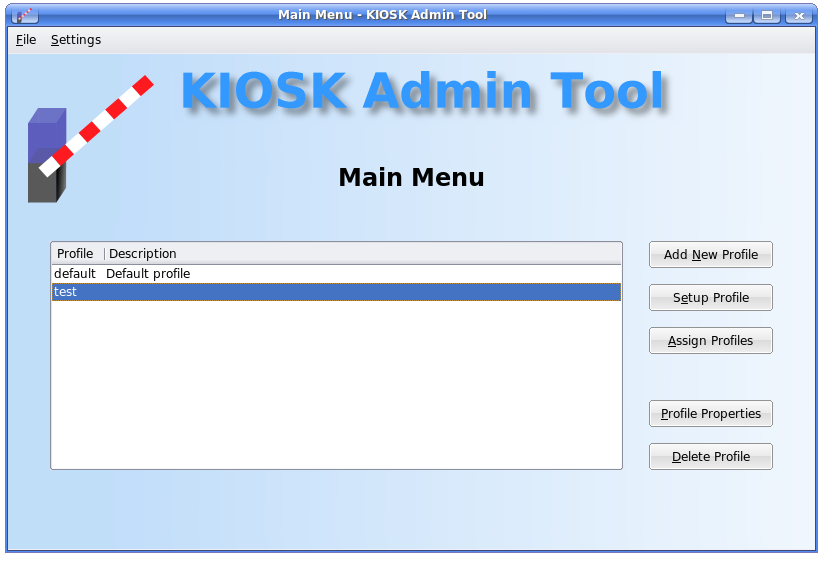
\includegraphics[width=10cm]{obrazky/KioskToolKDE3/uvodni_obrazovka.png}
    \caption{Úvodní obrazovka programu}
    \label{fig:kt3_uvodni}
\end{figure}
Úvodní obrazovka \ref{fig:kt3_uvodni} ukazuje seznam profilů s~jejich popisem, lištu s~menu a~tlačítka pro manipulaci s~profily. Velmi chybí možnost zkopírovat již existující profil.

\begin{figure}[h]
    \centering
    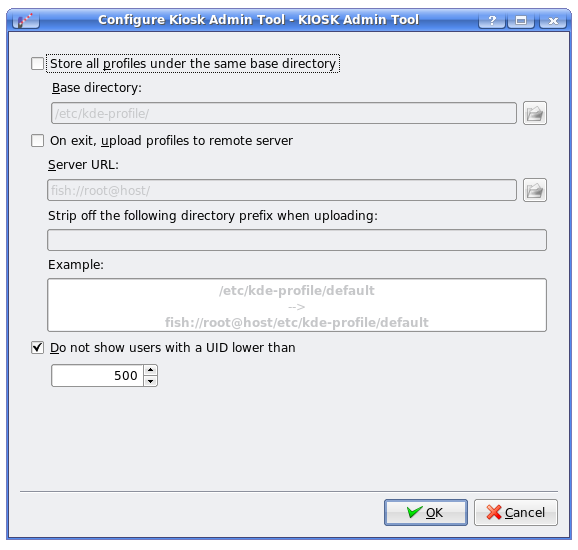
\includegraphics[width=10cm]{obrazky/KioskToolKDE3/nastaveni.png}
    \caption{Dialogové okno s~nastavením}
    \label{fig:kt3_nastaveni}
\end{figure}
Mezi nastavení programu \ref{fig:kt3_nastaveni} patří také možnost automaticky uložit profily na vzdálený server.

\begin{figure}[h]
    \centering
    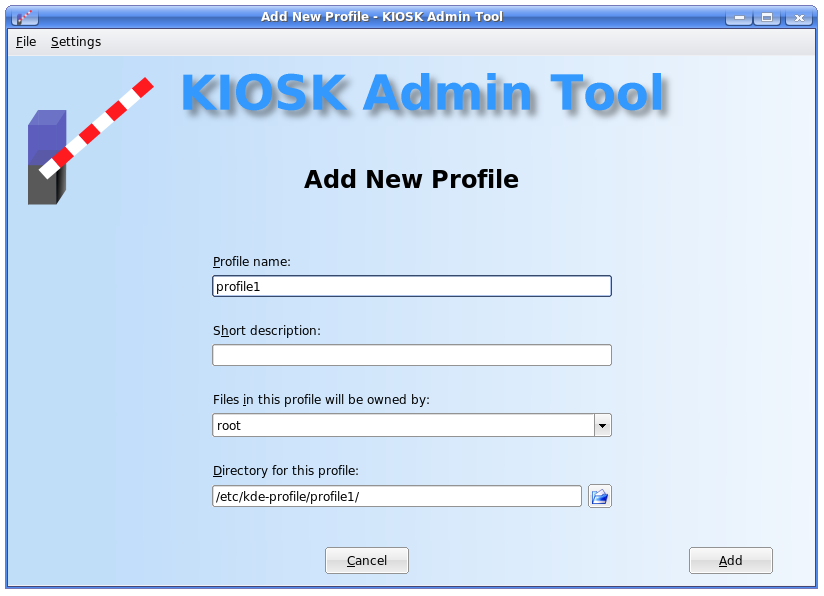
\includegraphics[width=10cm]{obrazky/KioskToolKDE3/novy_profil.png}
    \caption{Dialog pro vytvoření nového profilu}
    \label{fig:kt3_novyprofil}
\end{figure}
Dialog \ref{fig:kt3_novyprofil} pro vytvoření nového profilu je poměrně jednoduchý. Umožňuje nastavit název a~popis profilu a~dále který uživatel bude vlastnit složku s~profilem (bude mít přístup pro zápis) a~kde bude profil uložen.

\begin{figure}[h]
    \centering
    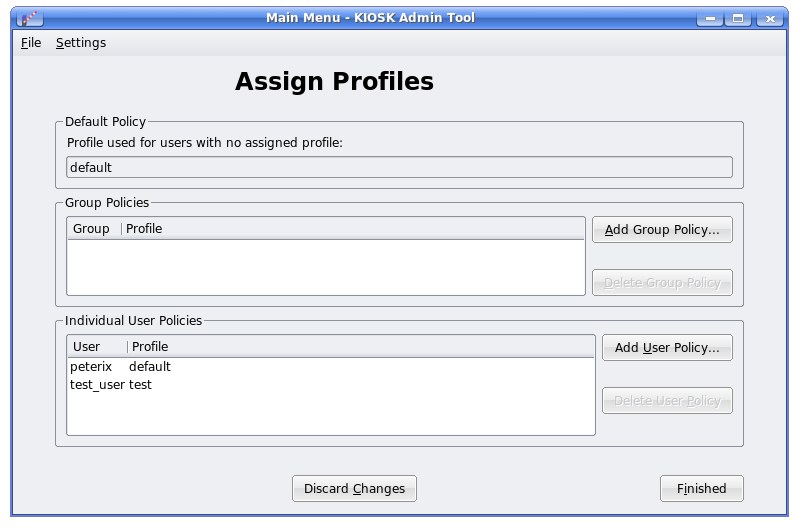
\includegraphics[width=10cm]{obrazky/KioskToolKDE3/prirazeni_profilu.png}
    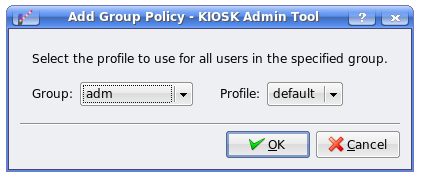
\includegraphics[width=8.5cm]{obrazky/KioskToolKDE3/prirazeni_profilu_skupine.png}
    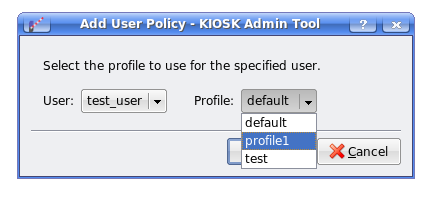
\includegraphics[width=8.5cm]{obrazky/KioskToolKDE3/prirazeni_profilu_uzivateli.png}
    \caption{Dialogy pro přiřazení profilů}
    \label{fig:kt3_prirazeni}
\end{figure}
Při pohledu na obrazovku a~dialogy pro přiřazení Kiosk profilů skupinám a~uživatelům je nutné si připomenout, že když má uživatel přiřazen svůj vlastní profil, nevztahují se na něj profily pro skupiny kterých je členem. To program nijak nezvýrazňuje. Bylo by dobré, kdyby poskytoval nějaký pohled, který by ukazoval všechny profily efektivní pro uživatele.

\begin{figure}[h]
    \centering
    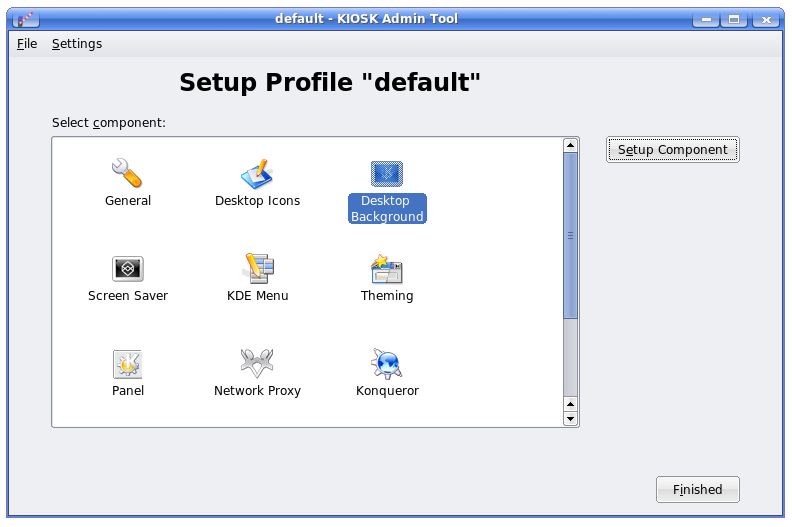
\includegraphics[width=10cm]{obrazky/KioskToolKDE3/seznam_komponent.png}
    \caption{Dialog s~nastavením profilu}
    \label{fig:kt3_nast_prof}
\end{figure}
Dialog \ref{fig:kt3_nast_prof} pro úpravu profilu je mnohem zajímavější. Je možné z~něj spouštět KControl moduly a~jiné části systému KDE a~tak docílit toho, že KioskTool může využít již existující funkcionalitu. Není proto nutné znovu \uv{vymýšlet kolo} a~uživatel pro nastavení Kiosk profilů používá stejné nástroje jako pro normální nastavení. Tato původní verze nástroje KioskTool definuje všechny moduly a~jejich vlastnosti v~jednom velkém XML souboru.

\begin{figure}[h]
    \centering
    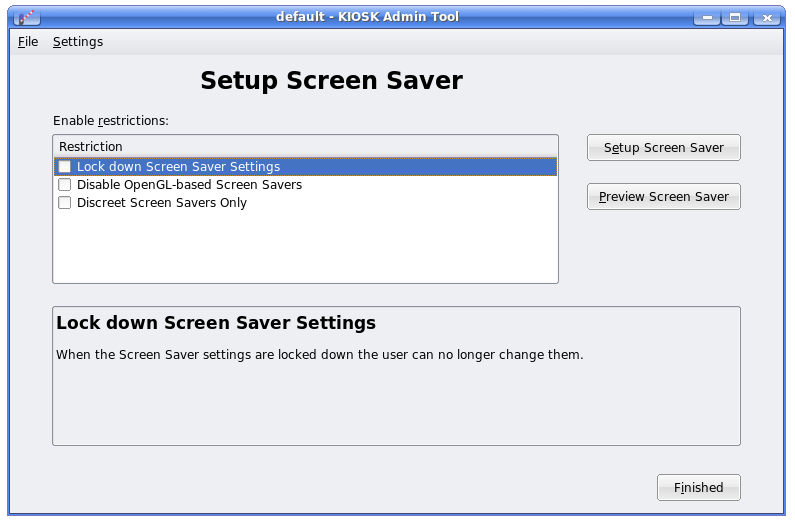
\includegraphics[width=10cm]{obrazky/KioskToolKDE3/ukazka_komponenty.png}
    \caption{Dialog jedné komponenty nástroje}
    \label{fig:kt3_nast_komp}
\end{figure}
Na obrázku \ref{fig:kt3_nast_komp} je vidět jak takový modul vypadá. Uživatel může zamknout obrázek na pozadí plochy a~ukázat si náhled tohoto obrázku (náhled ve smyslu, že se pozadí plochy dočasně zamění).

I~při krátké době nutné na seznámení s~nástrojem (KioskTool 1.0 v~Kubuntu 9.04) jsem narazil na fatální chyby, kdy se bez zjevného důvodu zhroutil. Nebude tedy možné se spolehnout na korektnost kódu.

\section{PolicyKit}
\begin{figure}[h]
    \centering
    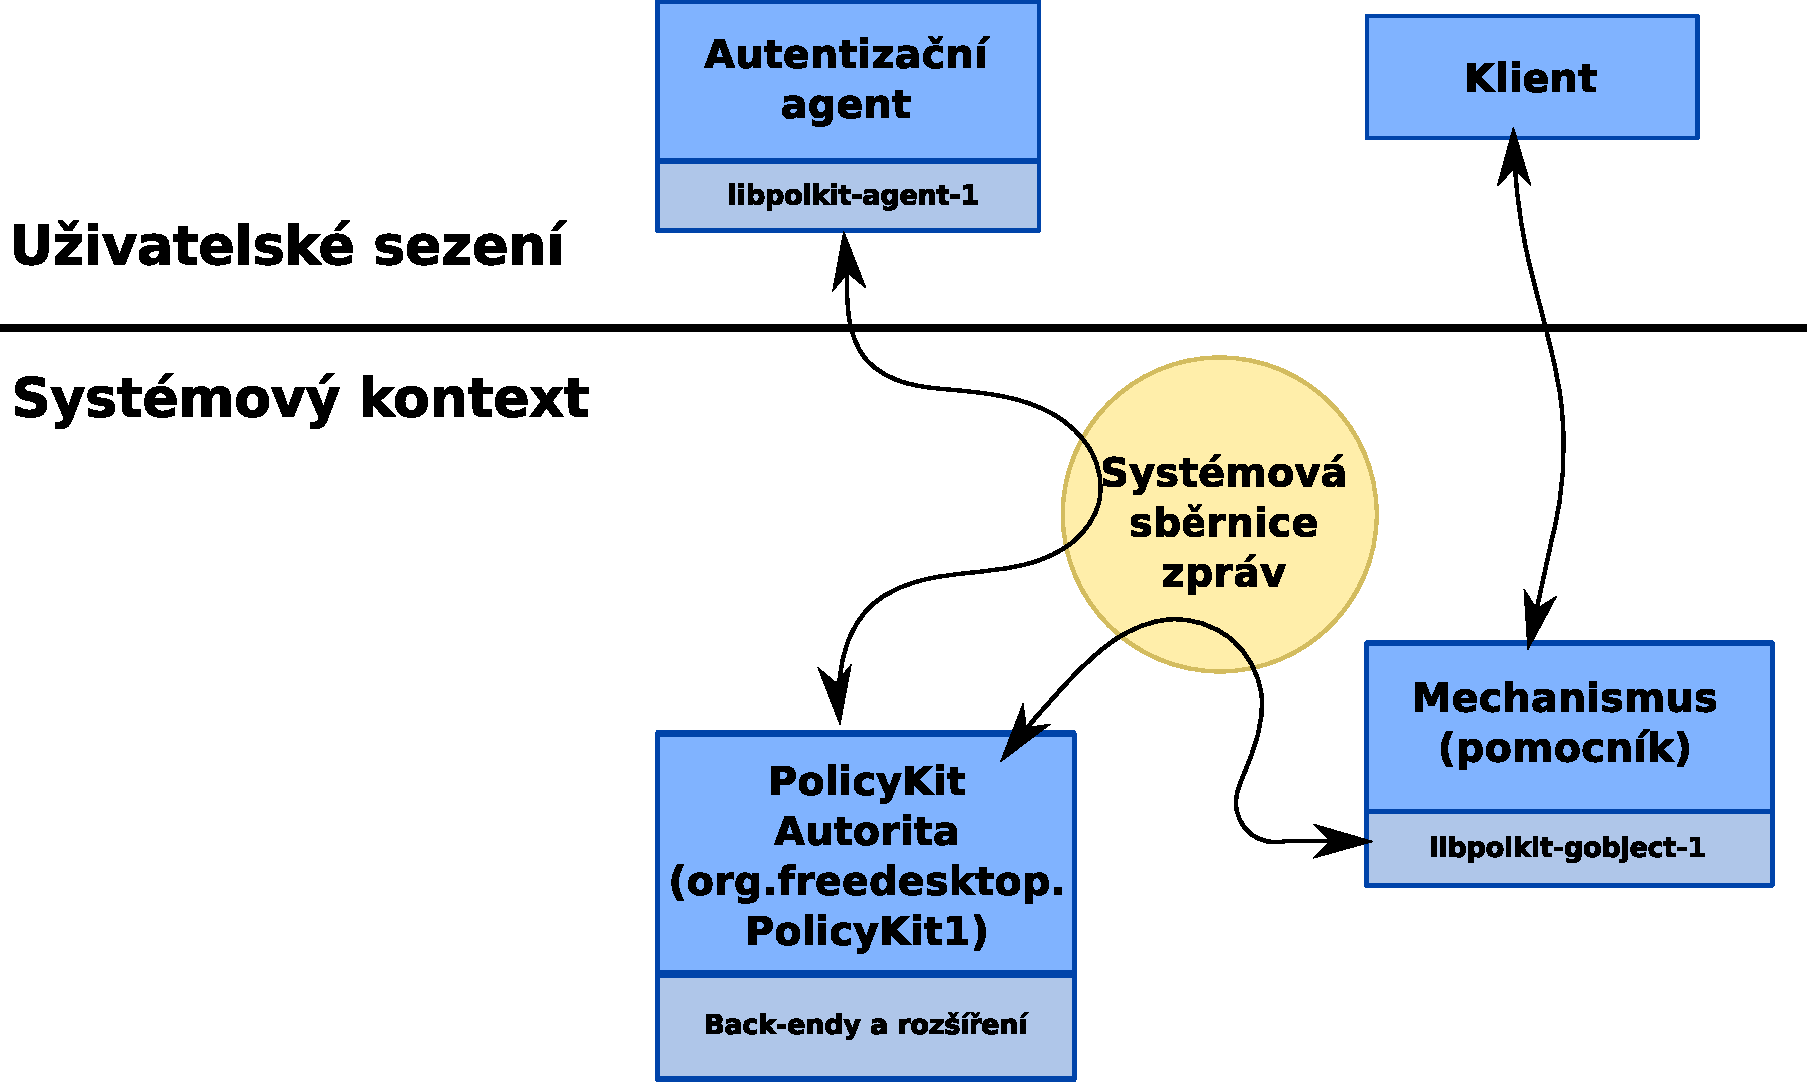
\includegraphics[width=12cm]{obrazky/polkit-architecture-vector-cz.pdf}
    \caption{Architektura systému PolicyKit, přeloženo z~\cite{manpolkit1}}
    \label{fig:polkit_arch}
\end{figure}

V~této sekci jsem čerpal z~manuálu \cite{manpolkit_overview}, převážně pak z~jeho částí \cite{manpolkit1} a~\cite{manpklocalauth}.

PolicyKit je systém umožňující autentizovat uživatele, autorizovat akce těchto uživatelů a~pomocí tzv. mechanismů tyto akce také provádět. Je to systém velmi modulární a~přenechává implementaci mnoha těchto funkcí zásuvným modulům a~programům které jej využívají. Pro každý typ rozšíření PolicyKitu existuje knihovna. Jednotlivé komponenty pak spolu komunikují pomocí IPC mechanismu D-Bus (ať už přímo nebo prostřednictvím knihoven).

Mezi nejzákladnější části tohoto systému patří démon polkitd, implementující část PolicyKit Authority. Ta se stará o~uložení databáze možných akcí a~povolení a~slouží jako centrální prvek celého systému.

Další částí, implementovanou prostředími jako je Gnome nebo KDE je tzv. autentizační agent. To je program, který například uživateli zobrazí okno pro zadání hesla, pokud je potřeba ověřit jeho totožnost. Pro samotné ověření je možné použít pomocný program běžící se superuživatelskými právy a~používající k~ověření systém jako je PAM -- ten je dobře popsán v~článku \cite{rootpam}. To ale není striktně vyžadováno. Lze i jen zobrazit obyčejné okno s~dotazem typu Ano/Ne.

Třetí komponentou je \uv{mechanismus} nebo \uv{pomocník}. zde se jedná o~službu pro vykonání privilegovaných akcí místo uživatele, který o~provedení akce žádá. Čtvrtou a~poslední komponentou je klient. To je program, který využívá služeb systému PolicyKit.
% http://lists.freedesktop.org/archives/polkit-devel/2009-July/000153.html

Průběh akcí v~systému pro volání funkce pomocníka může vypadat například takto:
\begin{itemize}
\item Uživatel se přihlásí, je nastartováno sezení KDE a~s~ním i autentizační agent
\item Autentizační agent se registruje u~PolicyKit autority
\item Uživatel spustí program, který využívá služeb PolicyKitu
\item Program zavolá funkci pomocníka přes systém D-Bus
\item DBUS démon nastartuje program pomocníka, pokud již neběží (pomocník musí být v~systému D-Bus registrován)
\item Spuštěný pomocník se zeptá PolicyKit autority, jestli je volaná akce autorizována
\item PolicyKit autorita zkontroluje, jestli je již tato akce autorizována (autorizace může mít například platnost po dálku celého sezení). Pokud není zatím autorizována, zjistí jakým způsobem se má autorizace dosáhnout.
\item Pokud je to nutné, zavolá PK autorita autentizačního agenta. Zobrazí se například okno, kde má uživatel zadat své login údaje. Je možné ověřovat buď pouze identitu uživatele, kdy stačí, že se přihlásí pod vlastním účtem, nebo je možné vyžadovat přihlášení účtu se superuživatelskými právy.
\item Uživatel se přihlásí. Záleží na tom jakým způsobem to agent dělá. Výchozí je PolicyKit mechanismus který obaluje PAM.
\item Agent oznámí autoritě jestli byla autentizace úspěšná.
\item Autorita vrací výsledek autorizace a~uloží si ho do vyrovnávací paměti po dobu její platnosti.
\item Pokud byl proces autorizace úspěšný, pomocník provede požadovanou akci.
\item V~tomto bodě může pomocník oznámit programu výsledek akce.
\end{itemize}

Toto samozřejmě není jediný možný průběh. Vše záleží na implementaci jednotlivých komponent. Jak jsem již uvedl, PolicyKit je velmi modulární systém a~většinu jeho částí lze nahradit nebo rozšířit.

Nad PolicyKitem je postavena knihovna polkit-qt. Poskytuje v~zásadě stejné funkce jako PolicyKit a~lépe je integruje do prostředí knihoven Qt.

Polkit-kde je nadstavbou nad knihovnou polkit-qt, která implementuje autentizační agent pro prostředí KDE a~KControl modul pro úpravu akcí povolených pro uživatele a~skupiny.

Zatím jediným způsobem uložení povolených akcí v~PolicyKitu je tzv. lokální autorita. Je to výchozí implementace PolicyKit Autority a~využívá lokálně uložených textových souborů s~příponou .policy a~.pkla. Nejdříve příklad \ref{fig:pkit_policy} .policy souboru. Tyto soubory používají formát XML a~vymezují seznam známých akcí. Instalují se do systému jako součást balíčků.

Značka \cppc{vendor} určuje k~čemu tento soubor akcí patří. V~tomto případě je to KControl modul pro nastavení data a~času. Soubor má dále nastavenu ikonu a~samotný seznam akcí. Akce má popis (description), zprávu pro případ neúspěšné autorizace (message) a~výchozí nastavení autorizace. PolicyKit rozlišuje mezi tzv. aktivním a~pasivním sezením. Aktivní je například normálně přihlášený uživatel s~vlastním X serverem. Pasivní může být sezení spuštěné dodatečně z~login terminálu (su - username). Normálně může být aktivní pouze jedno sezení (to s~kterým uživatel zrovna přímo pracuje). Soubor povoluje měnit nastavení času pouze uživateli s~aktivním sezením, který se prokáže jako superuživatel.

\begin{mylisting}
\caption{Ukázka souboru s~definicí akce (.policy soubor)}
\label{fig:pkit_policy}
\begin{lstlisting}[language=XML]
<?xml version="1.0" encoding="utf-8"?>
<!DOCTYPE policyconfig PUBLIC
"-//freedesktop//DTD PolicyKit Policy Configuration 1.0//EN"
"http://www.freedesktop.org/standards/PolicyKit/1.0/policyconfig.dtd">
<policyconfig>
<vendor>Date and Time Control Module</vendor>
<icon_name>preferences-system-time</icon_name>
   <action id="org.kde.kcontrol.kcmclock.save" >
      <description>Save the date/time settings</description>
      <message>System policies prevent you from saving the date/time settings.</message>
      <defaults>
         <allow_inactive>no</allow_inactive>
         <allow_active>auth_admin</allow_active>
      </defaults>
   </action>
</policyconfig>
\end{lstlisting}
\end{mylisting}

Takto hrubě vymezená práva a~omezení je dále možné pozměnit v~souborech .pkla. Efektivní seznam povolených akcí se získá sloučením těchto souborů. Je tedy možné mít například jeden soubor s~nastavením instalovaný z~distribučního balíčku a~druhý s~vyšší prioritou vytvořený administrátorem.

\begin{figure}[h]
    \centering
    \begin{verbatim}
               /var/lib/polkit-1
               └── localauthority
                   ├── 10-vendor.d
                   │   └── 10-desktop-policy.pkla
                   ├── 20-org.d
                   ├── 30-site.d
                   ├── 50-local.d
                   ├── 55-org.my.company.d
                   │   └── 10-org.my.company.product.pkla
                   └── 90-mandatory.d

               /etc/polkit-1
               └── localauthority
                   ├── 10-vendor.d
                   │   └── 01-some-changes-from-a-subvendor.pkla
                   ├── 20-org.d
                   ├── 30-site.d
                   ├── 50-local.d
                   ├── 55-org.my.company.d
                   │   └── 10-org.my.company.product.pkla
                   └── 90-mandatory.d\end{verbatim}
\label{fig:pkit_strukture}
\caption{Struktura složek pro PolicyKit Local Authority s~několika .pkla soubory. Převzato z~\cite{manpklocalauth}}
\end{figure}

Local Authority pro ně zavádí poměrně propracovanou strukturu \ref{fig:pkit_strukture}. Pořadí načítání je určeno lexikografickým řazením složek a~souborů v~nich. Pokud je stejně pojmenovaný soubor v~obou umístěních (ve /var/lib/ i /etc/), nejdříve se zpracuje ten ve /var/.

Ve struktuře \ref{fig:pkit_strukture} by pořadí zpracování vypadalo takto:
\begin{itemize}
\item 10-desktop-policy.pkla
\item 01-some-changes-from-a-subvendor.pkla
\item 10-org.my.company.product.pkla (z~/var)
\item 10-org.my.company.product.pkla (z~/etc)
\end{itemize}

\begin{mylisting}
\caption{Ukázka souboru s~nastavením PolicyKit Local Authority, Přeloženo z~\cite{manpklocalauth}}
\label{fig:pkit_pkla}
\begin{lstlisting}
[Povolene akce pro zamestnance]
Identity=unix-group:zamestnanci
Action=com.example.uzasnyprodukt.*
ResultAny=no
ResultInactive=no
ResultActive=yes

[Zakazy pro par cernych ovci]
Identity=unix-user:petr;unix-user:pavel
Action=com.example.uzasnyprodukt.*
ResultAny=no
ResultInactive=no
ResultActive=auth_admin
\end{lstlisting}
\end{mylisting}

Na výpisu \ref{fig:pkit_pkla} je ukázka .pkla souboru. Popíšu na něm, jakým způsobem se získá výsledek autorizace určité akce. Uživatelé petr a~pavel jsou členy skupiny zamestnanci.

Záznamy se zpracovávají tak jak jdou za sebou a~platí, že zpracování pokračuje i po úspěšném porovnání uživatelkého jména/skupiny s~těmi od žadatele. Jako příklad si vezmu uživatele petr, který požádá o~autorizaci akce \cppc{com.example.uzasnyprodukt.uzasnaakce}. Zaměstnanci mají tuto akci obecně povolenu bez nutnosti se přihlašovat v~první skupině souboru. Zpracování však pokračuje a~uživatel petr se bude muset pro úspěšnou autorizaci akce přihlásit jako administrátor.

Rozdíl mezi položkami \cppc{ResultAny}, \cppc{ResultInactive} a~\cppc{ResultActive} se nemusí zdát zjevný. \cppc{ResultActive} a~\cppc{ResultInactive} jsou výsledky akce pro aktivní a~neaktivní sezení -- podobně jako značka \cppc{allow_active} a~\cppc{allow_inactive} v~.policy souborech. \cppc{ResultAny} pak určuje výsledek pro oba typy sezení. Alespoň jedna z~těchto položek musí být přítomna. Hodnota položky udává jakým způsobem bude uživatel žádající o~autorizaci akce autentizován.

\section{KAuth}
KAuth je nové rozhraní pro autorizaci v~KDE. Je postaveno na již existujících rozhraních v~operačních systémech. V~OS na bázi Linuxu je to zpravidla PolicyKit, v~OSX pak framework Authorization Services. Podporu pro nová rozhraní je možné přidat pomocí zásuvných modulů.

Pomocí KAuthu je možné autorizovat akce uživatele. Zásuvný modul se stará o~veškeré ověřování akcí. Z~pohledu PolicyKitu je zde aplikace používající KAuth v~roli klienta.

Další funkce -- a~možná nejdůležitější a~nejlépe fungující -- poskytovaná KAuthem je vytvořit pokud možno co nejjednodušší program, který pak bude v~odpověď na autorizovanou akci spuštěn příslušným autorizačním rozhraním. Takovýto program se nazývá KAuth pomocník (helper). Pomocník a~aplikace která ho využívá mohou do jisté míry komunikovat oběma směry a~je také možné sledovat průběh dlouho trvající akce uvnitř pomocníka. KAuth pomocník je rozšířením PolicyKit pomocníka o~tyto zjednodušené komunikační funkce. Hlavní výhodou je, že za použití pomocníka lze provádět privilegované akce bez nutnosti být přihlášen pod administrátorským účtem nebo tohoto účtu používat ke spuštění aplikace jako celku.

Další službou KAuthu je registrace pomocníků a~akcí v~jeho jednotlivých zásuvných modulech. Uživatel KAuthu tedy specifikuje, jaké akce a~pomocníky chce použít a~při kompilaci budou tyto specifikace převedeny do formy srozumitelné pro jeho zásuvné moduly - např. PolicyKit nebo OSX Authorization Services.

KAuth nepodporuje provádění změn v~seznamu platných akcí po kompilaci. Také neumožňuje měnit autorizované uživatele a~skupiny pro akce -- to je zcela přenecháno systémům pro autorizaci, které využívá. V~případě PolicyKitu je toto nastavení realizováno v~KControl modulu, který používá přímo knihovnu polkit-qt. Další nepodporovanou částí je jakákoliv idea bezpečnostních profilů přiřazovaných uživatelům a~skupinám. Nic takového konec konců není ani v~PolicyKitu, který byl KAuthu modelem. Toto jsou celkem závažné nedostatky, které budu muset nějak vyřešit.

Největším omezením je však omezení na názvy KAuth akcí. Od rozhraní nad kterými funguje zdědil všechna jejich omezení v~tomto směru. Pro jména akcí je tedy možné použít jenom malá písmena anglické abecedy, číslice a~tečku jako oddělovač. Specifikace akcí v~.actions souborech je také dále omezená tím, že všechny akce musejí mít společný základ (jmenný prostor).

Uvedu příklad .actions souboru \ref{fig:kauth_dotactions}. Tento byl použit k~vygenerování podobného souboru pro PolicyKit, který byl uveden dříve zde: \ref{fig:pkit_policy}.

\begin{mylisting}
\caption{Ukázka KAuth .actions souboru}
\label{fig:kauth_dotactions}
\begin{lstlisting}
[Domain]
Name=Date and Time Control Module
Icon=preferences-system-time

[org.kde.kcontrol.kcmclock.save]
Name=Save the date/time settings
Description=System policies prevent you from saving the date/time settings.
Policy=auth_admin
Persistence=session
\end{lstlisting}
\end{mylisting}

Soubor obsahuje skupinu Domain, která popisuje ke které aplikaci patří (V~tomto případě KControl modul pro nastavení data a~času) a~jakou má mít ikonu. Textové položky mohou být lokalizovány a~velkou většinu jsem zde vynechal.

Po skupině Domain následují definované akce. Platí, že název akce je také názvem skupiny v~souboru. Název akce se skládá ze dvou částí -- jmenného prostoru a~názvu akce v~něm. Zde je jmenným prostorem část \cppc{org.kde.kcontrol.kcmclock}. Název akce je \cppc{save}. Skupina dále obsahuje srozumitelný název (\cppc{Name}), popis (\cppc{Description}) a~výchozí chování při pokusu o~autorizaci.

Položka Policy určuje průběh autorizace. V~případě, že je nastavena na hodnotu \cppc{yes}, je autorizace okamžitá. \cppc{no} naopak znamená, že akce nemůže být autorizována. Pokud je nastavena na \cppc{auth_self}, bude akce autorizována pokud se uživatel přihlásí pod svou vlastní identitou -- ověří se tak, že je to opravdu on. Konečně \cppc{auth_admin} znamená, že akce bude autorizována pokud se uživatel přihlásí jako administrátor.

Poslední položkou skupiny je \cppc{Persistence}. Ta je nepovinná a~udává, na jak dlouho bude autorizace udělena. Možnostmi jsou \cppc{session}, kdy bude platit dokud se neodhlásí a~\cppc{always}, kdy nebude omezena.

\chapter{Integrace KAuth do KAuthorized}
První praktickou částí projektu je zjistit jak nejlépe integrovat systém KAuth do rozhraní KAuthorized. Toto není triviální úkol a~nějakou dobu mi trvalo, než jsem přišel na to, jak toho alespoň částečně dosáhnout. Začnu popisem dvou variant, které jsem musel pro závažné nedostatky zavrhnout (postupně jak jsem analyzoval jednotlivé  využitelné technologie). Třetí variantu, kterou budu implementovat, popisuji sekci \uv{Možné řešení}.

Když nepřihlédnu k~omezení KAuthu a~budu ho brát jako ideální systém pro autorizaci uživatelských akcí, vypadá vše poměrně dobře. Na jedné straně Kiosk, podporující uživatelské a~skupinové profily, změnu těchto profilů (stačí být superuživatelem a~upravovat profily standardními nástroji KConfigu).

Na druhé straně zatím neznámý autorizační systém. Ze zadání je však možno vyčíst, že jejich sloučení je možné. Dá se tedy předpokládat, že takový systém bude umět přidávat nové restrikce a~efektivně s~nimi pracovat, dále že bude mít nějakou podporu pro zmíněné uživatelské a~skupinové profily. Ideální by bylo, kdyby šlo specifikovat, jakým způsobem se budou slučovat a~jaké tedy budou konečné výsledky.

Můj první a~také nejjednodušší nápad byl vytvořit statický .actions soubor v~kombinaci s~integrací KAuth přímo do KAuthorized. V~zásadě by toto mohlo fungovat a~je to částí řešení. Není to ale celé řešení.

Problémem je zde to, že neexistuje definitivní seznam možných restrikcí akcí a~zdrojů v~Kiosk profilech. Toto by šlo řešit tak, že každý program KDE by tyto své akce a~zdroje specifikoval v~.actions souboru k~tomu určeném a~zahrnul by jeho překlad do svého sestavení. To ovšem vylučuje jakoukoliv možnost stejné úrovně podpory pro aplikace, které by takto akce nespecifikovaly.

Druhým problémem je neexistence možnosti nastavit autorizované akce pro uživatele a~skupiny pomocí KAuthu. Nejen že nejdou nastavit, KAuth navíc nemá ani žádné ponětí o~něčem, co by alespoň vzdáleně připomínalo způsob jakým se aplikují Kiosk profily. V~případě použití PolicyKitu tyto vcelku základní funkce nemá ve formě knihovny žádná vrstva - PolicyKit, polkit-qt, polkit-kde ani KAuth.

Druhý nápad byl takovýto: když KAuth nepodporuje nic z~toho, co by korektní implementace vyžadovala, bude nutné to nějak obejít, a~to co nejjednodušším způsobem.

Možným řešením je jednoduše se vzdát toho, že budeme mapovat akce mezi Kioskem a~KAuthem jedna ku jedné. Mělo by být přece možné umístit do KAuth pomocníka instanci KConfigu, která načte požadovaný Kiosk profil a~bude přes systém D-Bus umožňovat dotazování se na jednotlivé hodnoty v~nich. Bylo by také možné tyto hodnoty měnit. V~podstatě by to byl stále pouze KConfig, jen obalen v~pomocníkovi.

Problémy tohoto řešení nemusejí být zcela zjevné, pokusím se je ale popsat. Za prvé -- nezíská se tím vůbec žádná výhoda z~pohledu bezpečnosti. Kiosk profily musejí stále zůstat čitelné pro všechny uživatele, jinak by se při spuštění programů nemohly načíst a~části které nebudou takto integrovány v~pomocníkovi (vše s~výjimkou omezení akcí a~zdrojů ) by tím by byly zcela neefektivní.

Odpadá tak výhoda KAuthu, kde jak seznam restrikcí, tak jaké restrikce pro koho platí může být skryt před uživateli. Například při použití PolicyKit Local Authority je možné nastavit všechny soubory čitelné jenom superuživatelem.

Za druhé -- KAuth pomocníci mají omezenou životnost. Pokud nejsou využíváni po dobu deseti vteřin, jsou ukončeni (viz. zdrojový kód KAuth). Znamená to znovu načíst celý KConfig objekt. I~když je toto načítání vysoce optimalizováno, stále je vcelku zbytečné načítat celou konfiguraci dvakrát - jednou v~programu, který by volal KAuthorized a~podruhé v~KAuth pomocníkovi. Sdílet zde jeden objekt například umístěním do společné paměti by byl holý nesmysl, takže se taková věc ještě více prodraží.

Jedna z~vlastností KAuthu, kterou by se tak nedalo využít jsou srozumitelné názvy akcí v~systému. Místo \cppc{org.kde.kiosk.action.help} a~mnoha dalších by byly v~systému jen akce pomocníka. V~tom případě ne nedá mluvit o~integraci KAuthu a~KAuthorized.

Jsou tu i další problémy -- KAuth podporuje použití pomocníků pouze v~kombinaci se systémy PolicyKit a~D-Bus. Uživatelé Windows a~OSX mají smůlu. Tomu se asi nevyhneme.

Je vidět, že ani tudy cesta nevede. Jak tedy postupovat když se zadání zdá být nesplnitelné?

\section{Možné řešení}\label{mozres}
Řešení nebude až tak pěkné jak by mohlo být, kdyby KAuth podporoval zápis autorizací jakožto knihovní funkci. Stanovím zde některé základní podmínky, které integrace KAuth do KAuthorized musí splňovat a~omezení, která jsou daná implementací KAuthu. Některá je možné obejít, jiná bohužel ne.

Použití KAuthu by nemělo být povinné a~mělo by být zachováno chování rozhraní \cppc{KAuthorized} pokud možno tak, aby se z~pohledu aplikací nic nezměnilo. Zde je problém to, že administrátor může, ale také nemusí nastavit v~systému \cppc{KConfig} kteroukoliv položku jako nezměnitelnou. Pokud vložím kontrolu oprávnění pomocí KAuthu před kontrolu pomocí KConfigu, musím nějak zaručit, že omezení známá v~KAuthu mohou být brána jako změnitelná, tak aby mohly být dále modifikována pomocí nastavení v~KConfigu. Pokud vím, KAuth ani PolicyKit toto neumožňují. Musí se také počítat s~tím, že KAuth nemusí být funkční (je v~nové verzi použité v~této práci stále ještě nestabilní) nebo že konvertor zatím nikdy nebyl spuštěn a~v~těchto případech použít normální nastavení Kiosk profilu přes \cppc{KConfig}.

Dále je potřeba implementovat konvertor Kiosk profilů na nastavení lokálního systému pro autorizaci. Zde se budu muset držet PolicyKitu, protože jediný další podporovaný systém je Authorization Services v~operačním systému Apple OSX. Hardware potřebný pro legální provoz OSX bohužel nemám. Takovýto konvertor by měl umět běžet jak KAuth pomocník, tak i jako samostatný program spustitelný uživatelem z~příkazové řádky. Konverze z~Kiosk profilů bude jednosměrná, bude používat polkit-qt pro získání seznamu podporovaných omezení a~bude produkovat soubory .pkla, použitelné jen a~pouze v~PolicyKit Local Authority. Konvertor by mělo být možné, až bude stabilní, integrovat do KAuthu nebo balíku policykit-kde.

Dalším omezením konvertoru je, že pokud bude použita jiná autorita než PolicyKit Local Authority, konverze s~ní nebude fungovat. Ale vzhledem k~tomu, že tato autorita je výchozí, předpokládám že bude k~dispozici.

V~konvertoru je nutné zohlednit to, že postup aplikace profilů v~Kiosku je jiný než postup ověření autorizace v~PolicyKitu. Musí se 'nasimulovat' Kiosk a~jeho zvláštnosti, aby se nezměnilo chování KAuthorized.

Integrace KAuth do KAuthorized opět není triviální záležitostí -- je to sice otázka několika volání funkcí KAuth, ale autorizační funkce KAuthu na rozdíl od systémů na kterých staví nevrací chybové kódy v~případě, že akce neexistuje. Toto bude potřeba změnit.

Omezení na zdroje \cppc{KDE Resource Restrictions} si vyžádají změny ve třídě \cppc{KStandardDirs} -- bude potřeba umístit do jmenného prostoru \cppc{KAuthorized} funkci, která bude vracet seznam typů zdrojů s~nastaveným omezením.

Je také třeba zopakovat, že KAuth má některá omezení na názvy akcí. Všechny akce v~jednom .actions souboru musejí mít společný jmenný prostor a~v~PolicyKitu soubor musí být podle tohoto jmenného prostoru pojmenován. Navíc mohou názvy obsahovat pouze malá písmena latinky, číslice a~tečku jako oddělovač. Názvy akcí a~zdrojů v~Kiosku tato omezení samozřejmě nemají a~často využívají jiné znaky jako je například pomlčka, podtržítko nebo lomítko. Tyto znaky je potřeba buď odstranit nebo nahradit. Vzniká tak reálná možnost kolize názvů.

Otázkou tedy je zda má vůbec smysl pokračovat. Rozhodl jsem se, že implementuji alespoň to co půjde, abych lépe demonstroval nemožnost celé věci v~testovací fázi.
\section{Změny v~KAuthu}
Jak jsem již zmínil v~sekci \ref{mozres}, je potřeba rozšířit KAuth tak, aby vracel vedle informace o~úspěšnosti autorizace také zvláštní hodnotu pro případ, že akce není použitému systémem pro autorizaci známa. Důvodem je, že  Všechny systémy, které KAuth podporuje umožňují toto zjistit a~neměl by být tedy problém tuto vlastnost so KAuthu přidat.
\subsection*{PolicyKit a~Policykit1}
Tyto systémy jsou si velmi podobné. Ve výchozím stavu vypadá funkce pro získání autorizace takto: \ref{kauth-oldmethod}. Hodnota \cppc{Unknown} je vrácena v~případě, kdy dojde k~chybě během autorizace. Důvod chyby lze zjistit bližším dotazováním autorizačního rozhraní. Úprava metody pak vypadá takto: \ref{kauth-newmethod}.
\begin{mylisting}
\caption{Autorizace akce v~PolicyKit1}
\label{kauth-oldmethod}
\begin{lstlisting}[language=C++]
Action::AuthStatus Polkit1Backend::actionStatus(const QString &action)
{
    PolkitQt1::UnixProcessSubject subject(QCoreApplication::applicationPid());
    PolkitQt1::Authority::Result r =
        PolkitQt1::Authority::instance()->
        checkAuthorizationSync(action, &subject, PolkitQt1::Authority::None);
    switch (r) {
    case PolkitQt1::Authority::Yes:
        return Action::Authorized;
    case PolkitQt1::Authority::No:
    case PolkitQt1::Authority::Unknown:
        return Action::Denied;
    default:
        return Action::AuthRequired;
    }
}
\end{lstlisting}
\end{mylisting}
\begin{mylisting}
\caption{Autorizace akce v~PolicyKit1 po úpravách}
\label{kauth-newmethod}
\begin{lstlisting}[language=C++]
...
case PolkitQt1::Authority::Unknown:
    PolkitQt1::Authority::ErrorCode error =
        PolkitQt1::Authority::instance()->lastError();
    PolkitQt1::Authority::instance()->clearError()
    // E_CheckFailed should indicate that an action doesn't exist
    if(error == PolkitQt1::Authority::E_CheckFailed)
        return Action::Invalid;
    else // other errors. we treat them like before
        return Action::Denied;
...
\end{lstlisting}
\end{mylisting}
Při výsledku typu \cppc{Unknown} se zjistí, jestli byla chyba typu \cppc{E_CheckFailed} a~v~takovém případě se vrací hodnota \cppc{Action::Invalid}, která znamená, že jde o~neznámou akci.
\subsection*{OSX Authorization Services}
Tento framework umožňuje se přímo dotazovat na existenci akcí pomocí funkce \cppc{AuthorizationRightGet()}. Přidání podpory do KAuth je tak jednoduchou záležitostí přidání dotazu na existenci na začátek metody: \ref{osxverify}.
\begin{mylisting}
\caption{Ověření existence akce v~OSX Authorization Services}
\label{osxverify}
\begin{lstlisting}[language=C++]
Action::AuthStatus AuthServicesBackend::actionStatus(const QString &action)
{
    // check if the action exists first, return error if not
    OSStatus exists = AuthorizationRightGet(action.toUtf8(), NULL);
    if(exists != errAuthorizationSuccess)
        return Action::Invalid;
...
\end{lstlisting}
\end{mylisting}
%REF:http://developer.apple.com/mac/library/documentation/Security/Reference/authorization_ref/Reference/reference.html

\section{Přesun vyhodnocení omezení na zdroje do KAuthorized}
Zjišťování seznamu omezení na zdroje je umístěno v~metodě \cppc{addCustomized} třídy \cppc{KStandardDirs} a~tento seznam je vytvářen před tím, než se načtou Kiosk profily. Tato metoda přidává profily k~cestám pro načítání konfigurace a~třída \cppc{KComponentData}, která tuto metodu volá následně způsobí znovunačtení konfigurace. Z~takovéto načtené konfigurace ale již nejsou vytaženy seznamy omezení zdrojů.

Rozhodl jsem zjišťování seznamu omezených zdrojů přesunout do rozhraní \cppc{KAuthorized}, aby byly změny nutné pro integraci KAuthu pokud možno pouze na jednom místě.

Dále jsem se rozhodl, že oddělím zpracování tohoto seznamu od metody \cppc{addCustomized()} tak, aby se dalo spustit z~třídy \cppc{KComponentData} poté, co \cppc{KStandardDirs} přidá Kiosk profily mezi konfiguraci. Docílí se tím toho, že je možné uložit omezení zdrojů stejným způsobem jako omezení na akce.

Implementoval jsem tedy funkci \cppc{authorizeResourceTypes} pro získání seznamu omezení na zdroje ve formě objektu \cppc{QStringList} a~umístil ji do rozhraní KAuthorized. Dále jsem přesunul vyhodnocení těchto omezení do nové metody \linebreak\cppc{evaluateRestrictedResources()} v~\cppc{KStandarDirs}, která je volána po znovu-načtení konfigurace po přidání profilů. Bylo nutné také změnit konstruktor privátního objektu v~KAuthorized, aby neblokoval zpracování profilů. Původně nebyl navržen na to, aby byl použit tak brzo během spouštění programů.

\section{Specifikace omezení akcí a~zdrojů}
Ke specifikaci akcí v~systému KAuth jsou využity statické .actions soubory. Nevýhody tohoto řešení jsem již uvedl, ale jinak to nejde. Jako základní jmenný prostor jsem se rozhodl použít \cppc{org.kde.kiosk}. Pro akce jsem se rozhodl pro \cppc{org.kde.kiosk.action} a~pro zdroje \cppc{org.kde.kiosk.resource}.

Názvy akcí a~zdrojů nemohou obsahovat jiné znaky než malá písmena a~číslice. Je tedy nutné přeložit jejich skutečné názvy do formy, kterou je KAuth schopen použít. Z~akce \cppc{action/help} se tak stane \cppc{actionhelp}, společně se jmenným prostorem pak \linebreak\cppc{org.kde.kiosk.action.actionhelp}. Kdyby exitovala jiná akce s~názvem  \cppc{action\_help}, došlo by ke kolizi.

\section{Implementace konvertoru}
Konvertor se skládá ze dvou částí. Hlavní a~nejdůležitější částí je pomocník, postavený na knihovně KAuth. Ten implementuje veškeré funkce celku (ve zdrojovém kódu je to kdelibs/kdecore/auth/kioskpklahelper.cpp). Druhou částí je jednoduchý terminálový program, který není až na spuštění pomocníka přes KAuth příliš zajímavý (ve zdrojových kódech je to kioskpklaconvert.cpp ve stejné složce jako pomocník).

Konvertor funguje tak, že nejdříve získá ze souboru /etc/kde4rc nastavení Kiosku, pomocí něj vyhledá Kiosk profily, komu a~jakým skupinám jsou přiřazeny a~jaké je pořadí skupin při zpracování skupinových profilů. Je také získán seznam akcí známých v~PolicyKit1 Local Authority. Tento seznam se filtruje do dvou skupin podle jmenných prostorů použitých pro omezení na akce a~zdroje. Toto jsou základní vstupní parametry programu. Uživatel nemá možnost do procesu přímo zasáhnout -- program nemá žádné uživatelské vstupy.

Další částí je vytvoření .pkla souboru ze skupinových profilů. V~pořadí zjištěném z~nastavení Kiosku se z~nich pomocí KConfigu načtou soubory globálního nastavení kdeglobals. Z~těch jsou dále vytaženy skupiny \cppc{KDE Action Restrictions} a~\cppc{KDE Resource Retrictions}. Klíče jejich položek jsou zpracovány stejně jako specifikace v~.actions souborech. Upravené klíče společně s~jejich hodnotami a~přiřazenou skupinou pak tvoří záznamy ukládané do .pkla souboru pro skupiny. Soubor je uložen tak, aby byl zpracován dříve než soubory pro jednotlivé uživatele (jsou načítány v~lexikografické pořadí podle názvu).

Dalším bodem je zpracování profilů přiřazených uživatelům. Postup je z~části podobný jako u~bodu předchozího, ale platí, že na uživatele s~nastaveným uživatelským Kiosk profilem se skupinové profily nevztahují. Znamená to, že každý uživatel musí mít specifikovány všechny akce ve výchozím stavu (povoleno). K~tomu se dále přidávají omezení z~uživatelského profilu. Ve výsledku se tak vyruší vliv skupinových profilů -- pro ilustraci: \ref{fig:konv_profily}. Pro každého uživatele je zvlášť vytvořen .pkla soubor.

\begin{figure}[h]
    \centering
    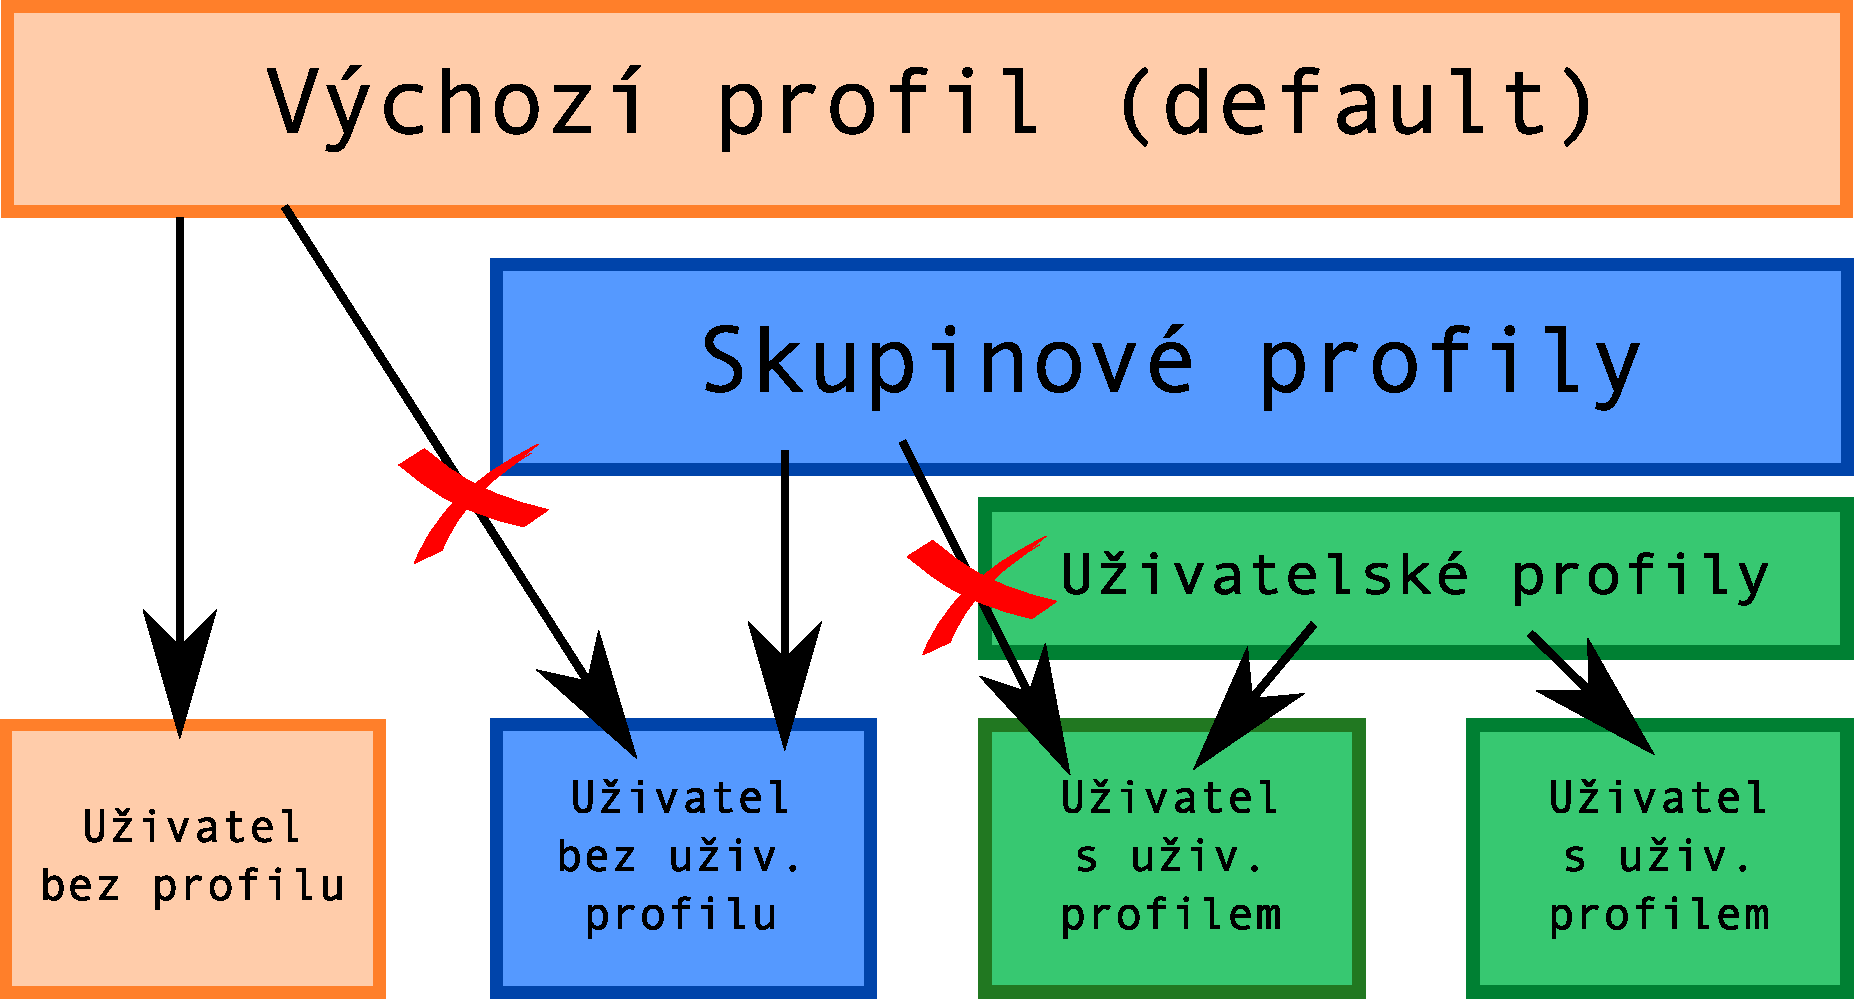
\includegraphics[width=8.5cm]{obrazky/profily.pdf}
    \caption{Aplikace Kiosk profilů}
    \label{fig:konv_profily}
\end{figure}

Problémem řešení je zejména nemožnost reprezentace vlastnosti nezměnitelnosti z~KConfigu. Omezení jsou jednou specifikována jako hodnota ano/ne v~nastavení PolicyKit Local Authority a~jsou tak z~pohledu KConfigu nezměnitelná. Jedinou možností jak docílit toho, aby byla změnitelná je nezanést ji do PolicyKitu. Pak ale není možné s~nimi v~něm pracovat. Když je jednou akce jako \cppc{action/help} pro ukázání menu s~nápovědou zanesena do KAuthu, ztrácí nad ní uživatel kontrolu a~nemůže tak menu schovat. To je poměrně závažný nedostatek.

% svn://svn.kde.org/home/kde/trunk/extragear/base/polkit-kde-1/
\section{Integrace KAuth do KAuthorized}
K~dokončení integrace zbývá už pouze jediný krok -- volat z~rozhraní KAuthorized metody systému KAuth. To se ukázalo být největším problémem ze všech. Vypadá to totiž, že KAuth zatím nikdy nebyl použit v~takto velkém rozsahu (autorizace všech akcí v~KDE). Není tedy překvapením, že tato integrace odkryla některé problémy v~KAuth a~jím implementovaném PolicyKitu.

KAuth nabízí několik možností, jak autorizovat akci. V~zásadě se jedná o~různé metody třídy \cppc{KAuth::Action}, mající mírně odlišný význam. Prvním metodou je \cppc{execute()} -- tato metoda je uvedena v~příkladu \cite{Kauth-usage} a~je určena pro jednorázové blokující provedení akce. Pokud je to potřeba, uživatel je požádán o~autentizaci. Metoda má podle \cite{Kauth-usage} fungovat i bez přítomnosti pomocníka. \cppc{execute()} má také asynchronní verzi.

Další metodou je \cppc{authorize()}. Tato metoda je určena pro získání autorizace pro akce před tím, než by byla akce provedena. Má být používána ostatními metodami třídy \cppc{KAuth::Action}.  Metoda podobně jako \cppc{execute()} může od uživatele vyžadovat autentizaci. Třetí metodou je \cppc{status()} -- tato metoda je podobná \cppc{execute()}, ale v~případech, kdy by byla vyžadována autentizace pouze o~této skutečnosti
informuje.

Takovýto význam by alespoň tyto metody měly mít. Skutečnost je ale odlišná. \cppc{KAuth::Action} používá pro autentizaci a~použití pomocníků statické zásuvné moduly -- to znamená, že jsou určeny při sestavení. Tyto moduly implementují lokálně dostupné autentizační mechanismy. Zde vzniká problém kvality těchto mechanismů a~jejich implementace v~KAuthu. To je také hlavním kamenem úrazu. Mnou používaný PolicyKit1 například vůbec neimplementuje metodu \cppc{authorize()}. Ta namísto výsledku vždy vrací hodnotu \cppc{Action::Authorized}. Její místo zastává metoda \cppc{status()}, která obaluje metodu \cppc{checkAuthorizationSync()} z~knihoven polkit-qt-1. Toto je synchronní metoda pro autorizaci uživatele, která umožňuje upravit zda bude vyžadovat od uživatele autentizaci příznakem. Proč není implementována metoda \cppc{authorize()} je nejasné.

Ze všech uvedených metod je nejvhodnější, alespoň podle komentářů v~kódu, metoda \cppc{status()}. Po konverzi z~Kiosk profilů totiž nevznikají akce pro jejichž autorizaci by bylo nutné se autentizovat. Při použití této metody v~kombinaci s~PolicyKitem však dochází k~nežádoucím jevům. Program, který používá takto upravené rozhraní KAuthorized totiž po čase \uv{zamrzne}. To stejné se stane i s~celým sezením KDE. Zkoušel jsem použít i jiné metody, ale výsledky byly ještě horší.

Pro zjištění kde je chyba jsem vytvořil jednoduchý test kauthDoS. Ten v~nekonečném cyklu volá \cppc{KAuth::Action::status()} a~v~pravidelných intervalech vypisuje hlášení. Když program přestane vypisovat, znamená to, že došlo k~chybě. Démon polkitd a~program kauthDoS byly spuštěny v~debuggeru gdb a~byly získány \uv{backtrace} z~obou programů (výpisy \ref{btrac1} a~\ref{btrac2}). Podle těch to vypadá, že problém vzniká během komunikace jednotlivých částí PolicyKitu. Chybu jsem ohlásil jeho autorovi (David Zeuthen) a~čekám na odpověď.

\begin{mylisting}
\caption{Backtrace z~démona polkitd při 'zamrznutí' (zkrácený)}
\label{btrac1}
\begin{lstlisting}
#0  poll () from /lib/libc.so.6
#1  in socket_do_iteration () from /usr/lib/libdbus-1.so.3
#2  in _dbus_transport_do_iteration () from /usr/lib/libdbus-1.so.3
#3  in _dbus_connection_do_iteration_unlocked () from /usr/lib/libdbus-1.so.3
#4  in _dbus_connection_block_pending_call () from /usr/lib/libdbus-1.so.3
#5  in egg_dbus_connection_pending_call_block (
       connection=0x61a990, pending_call_id=196205)
       at eggdbusconnection.c:2521
...      
#16 in g_main_context_dispatch ()
       from /usr/lib/libglib-2.0.so.0
#17 in g_main_context_iterate ()
       from /usr/lib/libglib-2.0.so.0
#18 in g_main_loop_run ()
       from /usr/lib/libglib-2.0.so.0
#19 in main ()
\end{lstlisting}
\end{mylisting}

\begin{mylisting}
\caption{Backtrace z~testovacího polkitd při 'zamrznutí' (zkrácený)}
\label{btrac2}
\begin{lstlisting}
#0  in poll () from /lib/libc.so.6
#1  in socket_do_iteration ()
    from /usr/lib/libdbus-1.so.3
#2  in _dbus_transport_do_iteration ()
    from /usr/lib/libdbus-1.so.3
#5  in egg_dbus_connection_pending_call_block (
    connection=0x6add50, pending_call_id=74401)
    at eggdbusconnection.c:2521
#6  in polkit_authority_check_authorization_sync ()
    from /usr/lib/libpolkit-gobject-1.so.0
#7  in PolkitQt1::Authority::checkAuthorizationSync ()
    from /home/kde-devel/kde/lib/libpolkit-qt-core-1.so.0
#8  in KAuth::Polkit1Backend::actionStatus ()
    at kdelibs/kdecore/auth/backends/polkit-1/Polkit1Backend.cpp:87
#9  0x000000000040162e in main (argc=1, argv=<value optimized out>)
    at kdelibs/kdecore/auth/kauthDoS.cpp:40 
\end{lstlisting}
\end{mylisting}
Systém KAuth za využití PolicyKit1 tedy do jisté míry funguje, není ale nijak spolehlivý. Co funguje dobře jsou pomocníci. Ti mají zpravidla několik málo akcí, které se používají pouze pokud je to nutné -- příkladem budiž KControl modul pro nastavení času, nebo mnou implementovaný konvertor pro Kiosk profily. Při integraci do rozhraní KAuthorized, které je využíváno téměř každým programem v~KDE je však objem dotazů o~několik řádů vyšší. Sezení KDE tak přestane reagovat již během spuštění. Chyba v~podstatě umožňuje přihlášenému uživateli provést DoS\footnote{Denial of Service} útok na PolicyKit, protože polkitd běží jako systémová služba, společná pro všechny uživatele. V~dalším testování tedy bohužel nelze smysluplně pokračovat, dokud nebude tato chyba odstraněna.

\section{Návrh dalšího postupu}
Výše byly popsány vybrané části rozhraní KAuthorized, KAuth a~PolicyKit. Nyní následuje návrh řešení v~nich nalezených nedostatků a~také návrh na jejich rozšíření. V~prvé řadě je potřeba opravit zmíněnou bezpečnostní chybu v~PolicyKitu.

Dále je potřeba rozšířit KAuth:
\begin{enumerate}
\item Je potřeba, aby uměl hlásit, pokud autorizovaná akce není známa -- a~to pro všechny podporované autorizační systémy. Toto jsem pro účely práce udělal a~otestoval pro metodu \cppc{status()} a~PolicyKit1. Ideální by bylo integrovat vyhledání akce do konstruktoru třídy \cppc{KAuth::Action} a~vracet pak výsledek pomocí volání její metody \cppc{isValid()}.
\item KAuth musí umět nejen ověřovat a~spouštět akce, ale také měnit oprávnění k~těmto akcím pro uživatele a~skupiny. Zde je zatím k~dispozici pouze KControl modul pro PolicyKit v~balíku policykit-kde-1 a~sním spojený pomocník na bázi polkit-qt-1, ale ten je zaměřen pouze na uživatele a~není nijak do KAuthu integrován.
\item Mělo by také být možné přidávat nové akce. To znamená, že by se nemusely do systému instalovat statické soubory s~definicemi akcí.
\end{enumerate}

Body 2 a~3 by bylo možné realizovat jakožto pomocníky a~přidat do systému KAuth rozhraní, které by umožnilo s~nimi pracovat.

Korektní integraci KAuthu přímo do KAuthorized považuji kvůli omezením ze strany KAuthu za nemožnou. I~když to tak na první pohled nevypadá, oba systémy jsou velmi rozdílné v~některých kritických bodech. I~kdyby byla integrace úspěšná, nezískalo by se tím téměř nic. Na pouhé dotazování se na to, jestli je uživateli dovoleno provádět nějakou akci není potřeba KAuth. Stačí jakákoliv databáze schopná uložit údaje ve formě klíč-hodnota. To však nebrání využití KAuthu tam, kde použití pomocníků poskytuje větší bezpečnost. Izolují se části programu vyžadující administrátorská práva od zbytku kódu. Z~pohledu administrátora je možnost udělit konkrétním uživatelům a~skupinám oprávnění tyto pomocníky spouštět snad největší výhodou řešení.

Dalším možným rozšířením by bylo nějakým způsobem spojit KAuth se systémy jako je SELinux\footnote{Security Enhanced Linux}. Zde by byla výhoda v~tom, že akce, které by jinak byly uživateli umožněny jde omezit na úrovni operačního systému. Využitelnost KAuthu by se tak rozšířila například na omezení spouštění programů a~použití knihoven (příkladem budiž KControl moduly) a~skutečné omezení zdrojů dat. Například pokud by měl uživatel zakázáno používat vlastní pozadí na plochu, bylo by zamezeno programu plasma-desktop načítat jiné obrázky, než ty instalované do systému administrátorem - a~to bez možnosti to obejít. Omezení na zdroje tak jak je v~KDE4 je v~porovnání s~takovým řešením v~podstatě bezzubé. Potom by mělo smysl odstranit některé typy omezení ze systému KConfig, a~přímo je integrovat do KAuth. Za jiných podmínek to však považuji za nesmysl.

Co se týče kombinace Kiosk, KAuthorized a~KConfig, je rozhodně co dohánět. Bylo by dobré tyto části KDE pročistit a~zdokumentovat. Zdvojení funkcí \cppc{KAuthorized::authorize()} a~\cppc{KAuthorized::authorizeKAction()} je poněkud chaotické a~vede ke zmatkům, kdy je jeden název akce používán s~funkcemi náhodně. \cppc{KAuthorized::authorizeKAction()} by měla přijímat jako parametr pouze reference typu KAction, aby se takovým zmatkům předešlo.

\chapter{Nástroj KioskTool}
Při psaní této kapitoly jsem hojně využíval knih \cite{StarchQt4} a~\cite{Ezust}. Obzvláště \cite{Ezust} je vhodným zdrojem informací, protože je volně dostupná.

Starší verze nástroje pro KDE3 je již popsána v~druhé kapitole. Tato kapitola bude tedy věnována portu na KDE4 a~jakým způsobem funguje. Navrhnu pro něj nové uživatelské rozhraní a~opravím chyby, aby bylo možné program začít používat.

\begin{figure}[h]
    \centering
    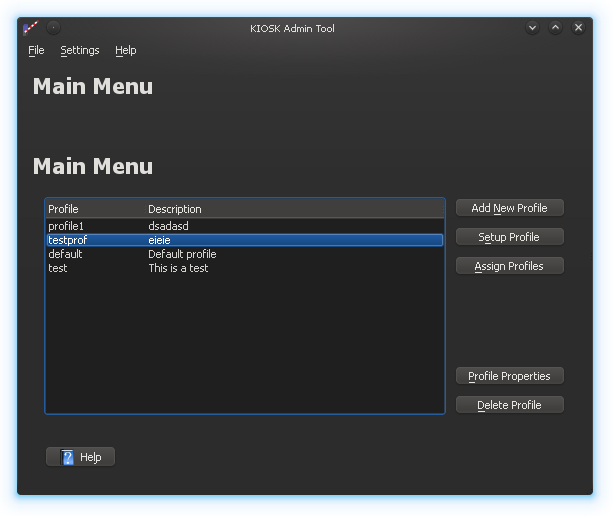
\includegraphics[width=10cm]{obrazky/KioskToolKDE4/kiosktool_kde4.png}
    \caption{Uživatelské rozhraní se od verze z~KDE3 příliš nezměnilo}
    \label{fig:kt4_uvod}
\end{figure}

Port nástroje do KDE4 totiž již existuje, i když je nedokončený a~dá se říci opuštěný. Uživatelské rozhraní se příliš nezměnilo: \ref{fig:kt4_uvod}. Původní nastavení pomocí velkého XML souboru bylo odstraněno a~nahrazeno mnoha menšími soubory (samozřejmě používají KConfig). To má za účel umožnit ostatím autorům napsat si pro své aplikace rozšíření. Nástroj však ztratil většinu svých starých vlastností, schopnost spouštět KControl moduly a~náhledy, své pěkné (i když zbytečné) obrázkové vzezření a~získal několik dalších chyb.

\paragraph{Strukturální popis}
Aplikace KioskTool se skládá z~několika základních komponent a~využívá grafické rozhraní navržené pomocí nástroj Qt Designer (části rozhraní jsou specifikovány v~.ui souborech, ze kterých se při kompilaci generuje kód). Vzhled je tedy alespoň z~pohledu programátora  částečně oddělen od funkce programu. Grafické prvky programu však přímo obsahují data se kterými se pracuje -- není využito návrhového vzoru MVC\footnote{Model-View-Controller}.

Při startu programu jsou nejdříve vytvořeny základní komponenty \cppc{KAboutData} a~\cppc{KApplication} a~hlavní komponenta grafického rozhraní \cppc{KioskGui}. Ta je zobrazena. Potom je nastartováno vyhodnocování událostí.

Komponenta \cppc{KioskGui} je odvozena od třídy \cppc{KXmlGuiWindow} -- načítá tedy část svého vzhledu z~.rc souboru \ref{listing:guirc} ve formátu XML.
\begin{mylisting}
\caption{kiosktoolui.rc}
\label{listing:guirc}
\begin{lstlisting}[language=XML]
<?xml version="1.0"?>
<!DOCTYPE gui SYSTEM "kpartgui.dtd">
<gui name="kioskgui" version="3.1">
<MenuBar>
 <Menu name="file">
    <Action name="upload_all"/>
 </Menu>
</MenuBar>
</gui>
\end{lstlisting}
\end{mylisting}

\cppc{KioskGui} potom vytváří instance tříd \cppc{KioskRun} a~\cppc{MainView}. \cppc{KioskRun} je pouhou obálkou nad souborem funkcí různého určení (tzv. God object anti-pattern) a~je používána pro většinu manipulace s~profily a~spouštění dalších programů. \cppc{MainView} pak určuje vzhled celého programu. Je to třída generovaná z~.ui souboru, obsahuje dvě úrovně nadpisů, tři tlačítka která mění význam podle kontextu a~objekt typu \cppc{QStackedWidget}, který je určen pro zobrazení aktuální stránky. Při startu je to stránka se seznamem profilů (\cppc{PAGE_PROFILE_SELECTION}).

Přechod mezi stránkami je prováděn pomocí metody \cppc{selectPage(enum page)}, volané v~reakci na akce uživatele a~lze v~hrubých obrysech popsat pomocí stavového automatu \ref{fig:kioskstates}.

\begin{figure}[h]
    \centering
    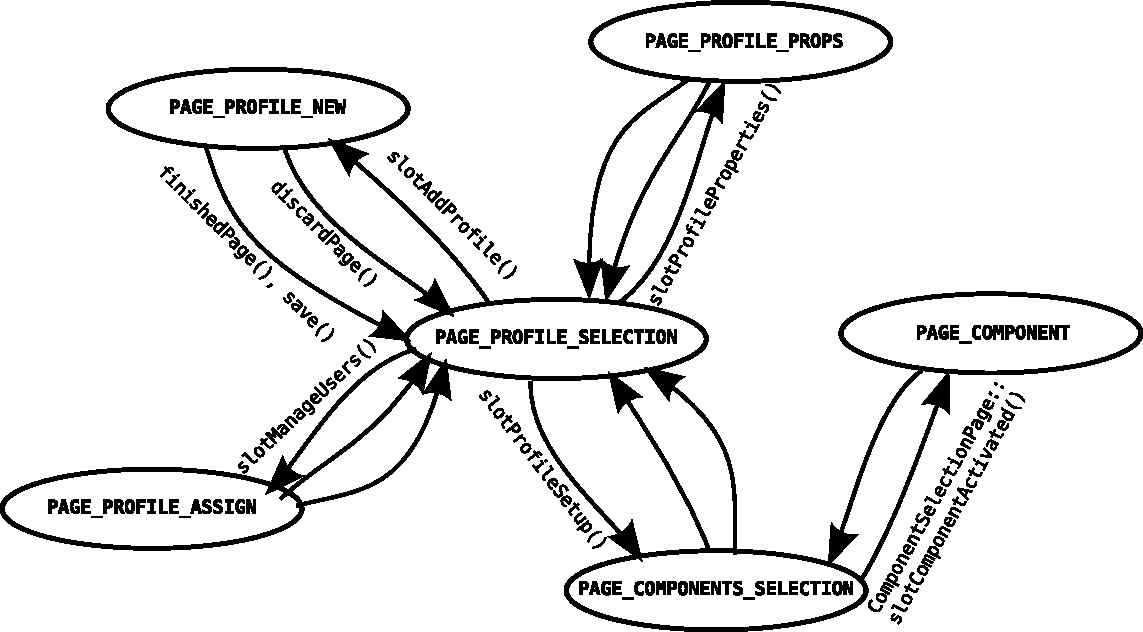
\includegraphics[width=10cm]{obrazky/stated.pdf}
    \caption{Stavy grafického rozhraní aplikace KioskTool}
    \label{fig:kioskstates}
\end{figure}

Ve stavech \cppc{PAGE_PROFILE_NEW} a~\cppc{PAGE_PROFILE_PROPS} je používán stejný typ stránky. Jednou pro vytvoření nového profilu, podruhé pro změny v~něm.\linebreak \cppc{PAGE_PROFILE_ASSIGN} je stav, ve kterém je aktivní stránka pro přiřazení profilů uživatelům a~skupinám. Ve stavu \cppc{PAGE_COMPONENTS_SELECTION} je načten profil a~je zobrazena stránka se seznamem komponent pro stav \cppc{PAGE_COMPONENT} -- zde přestává stačit jeden stavový diagram.

Je zřejmé, že způsob jakým je vytvořeno grafické rozhraní přímo určuje funkci programu. Přechod na stránku se seznamem komponent zapříčiní otevření profilu. Návrat na hlavní stránku se seznamem profilů pak způsobí jeho uložení. Platí to i naopak - technická omezení kladená na některé funkce programu se odrážejí v~návrhu jeho grafického rozhraní. Například program nemůže upravovat více jak jeden profil, protože ve třídě KioskRun nastavuje pro spuštění KConfig modulů proměnné prostředí a~kopíruje profil do dočasného umístění, kde ho může případná spouštěná aplikace měnit. Proto stavový automat a~přechody mezi stránkami. To by se mělo dát rozšířit -- program by měl např. být schopen pracovat s~profily na pozadí, zobrazovat okno pro úpravy konkrétního profilu (ať už vlastní nebo z~jiného programu) a~zároveň třeba i druhé okno se seznamem všech uživatelů a~k~nim přiřazených profilů. Je tedy potřeba oddělit model pro práci s~Kiosk profily a~jeho stavy od kódu pro grafické rozhraní.

Vzniká tak také nutnost práce s~asynchronními událostmi, protože provedení některých funkcí modelu může trvat déle než je přípustné a~blokovat tak uživatelské rozhraní. V~aplikaci, kde se pouze přechází mezi přesně vymezenými stavy je toto omluvitelné, ale pokud má uživatel otevřeno několik oken, nebude chtít například čekat, až se profil uloží na server.

Po těchto úpravách bude možné vylepšit uživatelské rozhraní programu. Stanovím si tedy několik cílů:
\begin{enumerate}
\item Krátkodobě - otestovat program a~opravit v~něm chyby, tuto verzi zveřejnit (bude součástí práce).
\item Navrhnout a~implementovat model pro práci s~profily. Měl by být bezpečný a~pro přístup k~profilům používat KAuth pomocníka. Nabízí se použít Qt API pro stavové automaty \cite{QtStatMach}.
\item Musí být možné upravovat profily zároveň z~více aplikací, případně ručně. KioskTool toto nijak neřeší a~je možné ztratit data pokud je spuštěn dvakrát.
\item Implementovat několik jednoduchých terminálových programů pro práci s~profily.
\item Nakonec vytvořit nové grafické rozhraní pro KioskTool.
\end{enumerate}

\paragraph{Triviální chyba}
Při testování jsem narazil pouze na jednu drobnou, ale závažnou chybu. Při přidělování profilů není možné přiřadit více jak jeden profil pro uživatele nebo skupiny. To znamená, že program není vůbec použitelný ke svému účelu. Problém má triviální řešení. Přiřazení se totiž řídilo tímto algoritmem:
\begin{lstlisting}[language=C++]
for( int idx = 0; idx < listGroups->topLevelItemCount(); ++idx )
{
    item = listGroups->topLevelItem(idx);
    if (item->text(0) == group)
        break;
}
if (item)
{
    Error();
\end{lstlisting}
To je zjevně špatné, protože proměnná item bude obsahovat nenulovou hodnotu, jakmile pude přiřazen alespoň jeden profil. Je tedy potřeba přidat za \cppc{break;} další řádek s~\cppc{item = 0;}. Tímto se stává program použitelným pro běžného uživatele.

\section{Návrh uživatelského rozhraní}
Zde je použit nástroj QtDesigner pro navržení vzhledu uživatelského rozhraní. Funkční část bude muset být dále implementována a~tento vzhled je nutno brát pouze jako první krok.

Namísto stránek a~stavových automatů bude mít program několik záložek. Zůstanou tedy tlačítka s~akcemi po stranách, ale uživatel bude mít mnohem větší přehled kde se nalézá. Seznam akcí také bude významně rozšířen.

\begin{figure}
\centering
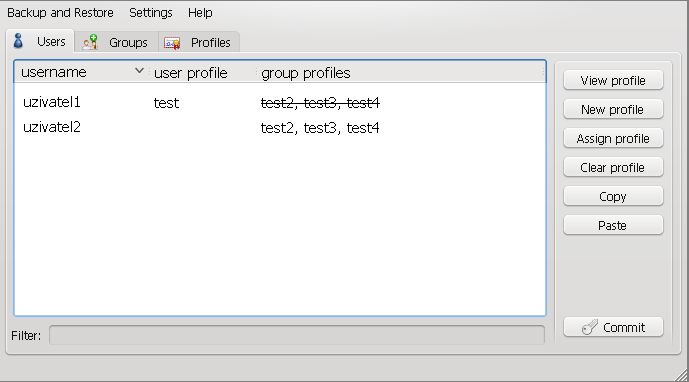
\includegraphics[width=10cm]{obrazky/navrh-usersz.png}
\caption{Karta pro uživatele}
\label{fig:kt4_newusers}
\end{figure}

Na obrázku \ref{fig:kt4_newusers} je program s~otevřenou kartou pro pohled na uživatele. Menu \uv{File} bylo nahrazeno menu \uv{Backup and Restore}, protože neobsahovalo nic jiného než akci pro zálohování profilů na server. Menu s~nastavením a~nápovědou zůstává. Většinu plochy programu zabírá pohled na seznam uživatelů a~k~nim přiřazených uživatelských a~skupinových profilů. Pokud má uživatel přiřazen jak uživatelský, tak skupinové profily, je zde fakt, že jsou ty skupinové neefektivní zvýrazněn přeškrtnutím.

V~seznamu po pravé straně je několik pro KioskTool nových akcí. Akce \uv{View Profile} slouží k~otevření okna s~profilem. Pokud má uživatel pouze skupinové profily, otevře se stejné okno, ale jeho obsah bude výslednicí skupinových profilů a~nebude možné jej měnit (toto musí být zvýrazněno aby nebyl uživatel programu uveden v~omyl). Akce \uv{View Profile} přiřadí uživateli nový prázdný profil. Akce \uv{Assign Profile} slouží k~přiřazení existujícího profilu uživateli. \uv{Clear Profile} odebere uživateli jeho profil.

Pod seznamem je pole pro filtrování uživatelů podle zadaného textu. Je tak možné rychle vyhledávat v~obsáhlém seznamu uživatelů.

\begin{figure}
\centering
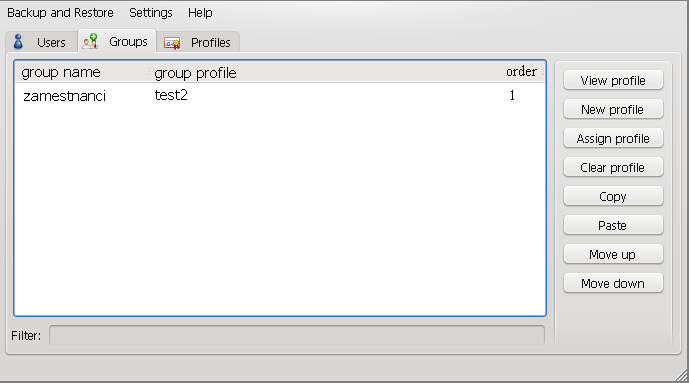
\includegraphics[width=13cm]{obrazky/navrh-groupsz.png}
\caption{Karta pro skupiny}
\label{fig:kt4_newgroups}
\end{figure}

Karta se skupinami \ref{fig:kt4_newgroups} je podobná kartě pro uživatele, zobrazuje však skupiny, jim přiřazené skupinové profily a~jejich pořadí. K~seznamu akcí z~karty s~uživateli jsou přidány akce pro změnu jejich pořadí. Pořadí by také mělo být možné měnit přetažením položek kurzorem na jinou pozici v~seznamu.

\begin{figure}[h]
    \centering
    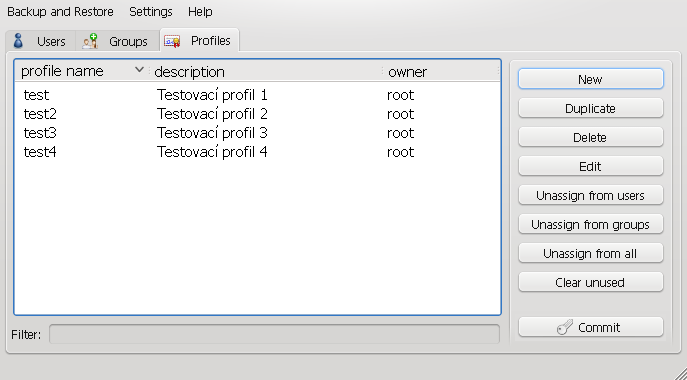
\includegraphics[width=13cm]{obrazky/navrh-profiles-fixd.png}
    \caption{Karta pro profily}
    \label{fig:kt4_newprofiles}
\end{figure}

Záložka s~profily \ref{fig:kt4_newprofiles} obsahuje jak název napovídá seznam profilů a~akce pro práci s~nimi. V~pořadí odshora vytvoření nového profilu, kopie již existujícího, smazání profilu, úpravu profilu a~dále akce pro zrušení přiřazení profilů pro uživatele, skupiny a~obojí zároveň. Seznam je zakončen akcí pro smazání všech nepoužívaných profilů.

Všechny záložky budou používat stejný model pro naplnění seznamů. Všechny také mají akci pro uložení změn \uv{Commit}. Při jejím použití by se měl zobrazit seznam všech uživatelem provedených změn a~umožnit tak uživateli je ještě jednou zkontrolovat před zapsáním na disk.

Změny v~profilech samotných by bylo dobré provádět způsobem podobným jako využívá nástroj KConfigEditor. Ten vypadá zhruba takto: \ref{fig:kconfeditor}. KConfigEditor používá rozšíření systému KConfig o~deklarace klíčů pomocí systému KConfigXT. Ten je zpravidla používán k~vygenerování dialogů pro nastavení programů. V~souboru KConfigXT se uvede jaké klíče z~konfigurace program používá a~také jejich typ. Navíc se tyto soubory instalují společně s~programy -- lze jich tedy využít v~editoru nastavení. Integrace tohoto nástroje a~rozšíření a~oprava KConfigXT souborů by pak vedly k~vcelku elegantnímu řešení problému úpravy profilů.

\begin{figure}[h]
    \centering
    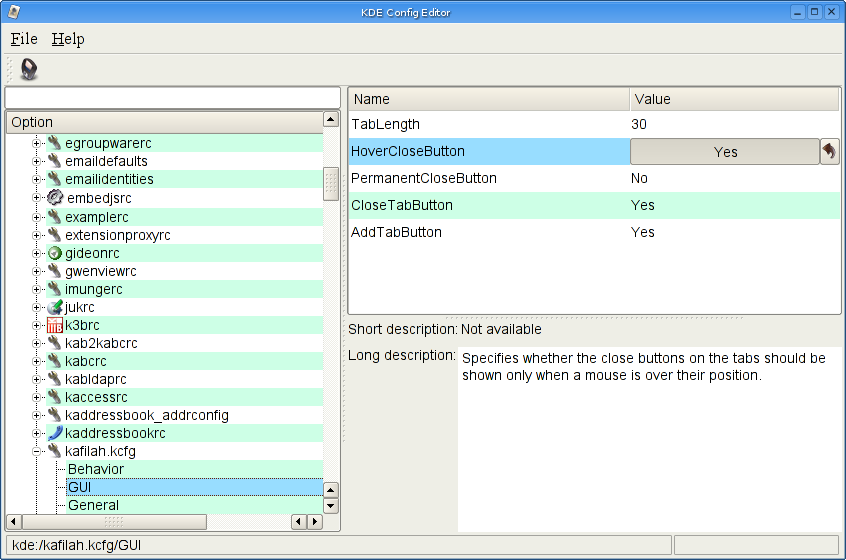
\includegraphics[width=10cm]{obrazky/kconfigeditor1.png}
    \caption{Ukázka programu KConfigEditor. Převzato z~\cite{KConfigEditor}.}
    \label{fig:kconfeditor}
\end{figure}

\chapter{Závěr}
V~kapitole 2 byly popsány technologie a~rozhraní, na kterých je dále stavěno.

V~kapitole 3 byl učiněn neúspěšný pokus o~integraci KAuth do KAuthorized. Byly přitom odkryty závažné nedostatky v~KAuth a~rozhraních, nad kterými je postaven. Nejzajímavější je pak Denial of Service útok na PolicyKit. Ten jsem objevil za pomoci implementovaného testovacího nástroje kauthDoS. KAuth byl integrován do KAuthorized, ale díky zmíněné chybě se při jeho použití stává prostředí KDE naprosto nepoužitelným. Začlenění tohoto celku do kdelibs tedy není z~praktických a~bezpečnostních důvodů vhodné a~proto jsem poslední bod zadání přeskočil.

Dále byl implementován nástroj kioskpklaconvert a~KAuth pomocník kioskpklahelper. Ty umožňují konvertovat omezení akcí a~zdrojů z~KConfigu do nastavení PolicyKit Local Authority.

Kapitola 4 popisuje port nástroje KioskTool do KDE4, navrhuje pro něj nové grafické rozhraní a~také popisuje provedené změny nutné pro zprovoznění nástroje. Tím je také splněn čtvrtý bod zadání. V~práci započaté na nástroji KioskTool budu pokračovat.

V~příloze B jsou informace o~umístění zdrojových kódů, obsahu přiloženého datového nosiče a~instalaci a~zprovoznění KDE4.

%=========================================================================
\appendix
\chapter{Vymezení pojmů}
\begin{description}
\item[Authorization Services] je obdoba PolicyKitu pro operační systém Apple OSX.
\item[KAuth] je rozhraní nad autorizačním řešením jako je například PolicyKit.
\item[KAuthorized] je tenké rozhraní nad KConfigem/Kioskem umožňující dotazování, zda jsou některé typy akcí povoleny.
\item[KConfig] je systém pro ukládání a~načítání nastavení v~KDE.
\item[KConfigXT] je systém pro uložení metadat pro systém KConfig. Popisuje klíče použité v~jednotlivých programech a~jejich typy.
\item[KControl modul] je modulem pro nastavení určité části KDE -- například rozložení klávesnice, vzhled oken, apod.
\item[Kiosk] je souhrnný pojem pro některé vlastnosti KConfigu a~postup načítání konfigurace obecně.
\item[Kiosk profil] je přiřazený uživateli nebo skupině uživatelů. Má vyšší prioritu než normální uživatelská nastavení KDE, ale nižší než globální systémové nastavení.
\item[KioskTool] je aplikace pro správu Kiosk profilů. V~KDE 3 umožňovala jednoduše nastavit některé aspekty Kiosku/KConfigu bez nutnosti měnit profily ručně.
\item[KDE] je komunita vývojářů pracujících na tzv. KDE Software Compilation. Zde používám označení KDE ve starém významu -- jako uživatelské prostředí.
\item[PolicyKit] je starší verze autorizačního rozhraní dostupná v~Linuxu.
\item[PolicyKit1,] nebo také "polkit" je jeho novější verze. Právě tu budu převážně používat.
\item[PolicyKit autorita] je centrálním prvkem systému PolicyKit. Slouží pro uložení autorizačních dat.
\item[PolicyKit Local Authority] je výchozí implementace PolicyKit autority. Používá textové soubory.
\item[polkit-qt] je soubor knihoven obalující PolicyKit.
\item[polkit-kde] je nadstavba nad polkit-qt pro prostředí KDE. Implementuje autentizačního agenta a~KControl modul pro práci s~autorizacemi.
\item[polkitd] je systémová služba PolicyKitu a~implementuje tzv. autoritu.
\item[Qt] je balík knihoven v~jazyce C++.
\item[QtDesigner] je program pro vizuální návrh uživatelského rozhraní programů na bázi Qt knihoven.
\end{description}
%=========================================================================
\chapter{Dodatečné informace}
\paragraph{Umístění zdrojových kódů}
Zdrojové kódy KDE4 a~jeho knihoven je možné prohlížet na adrese http://websvn.kde.org/trunk/KDE/. Většina práce byla vytvořena jako součást balíku kdelibs a~byla vyvíjena proti SVN revizi 1125098.

Přiložené datové médium obsahuje patch pro kdelibs, ve kterém jsou implementovány změny z~třetí kapitoly.
Kód čtvrté kapitoly je ve složce kiosktool.
Další informace k~obsahu média jsou v~souboru README.

\paragraph{Instalace - Integrace KAuth do KAuthorized}
Instalace kódu z~třetí kapitoly pravděpodobně nebude triviální.

\noindent
Základem je dokumentace na adrese http://techbase.kde.org/Getting\_Started/Build/KDE4. Pokud se KDE instaluje do domovského adresáře k~tomu vytvořeného uživatele, je nutné přihlédnout k~tomu, že registrační soubory KAuth pomocníků pro systém D-Bus a~soubory s~definicemi akcí pro PolicyKit je třeba překopírovat do systémových adresářů. Bez toho nemůže KAuth fungovat.

\noindent
Konkrétně je nutné překopírovat tyto soubory:

\noindent
Vše z~\cppc{\$prefix/etc/dbus-1/system.d} do \cppc{/etc/dbus-1/system.d}

\noindent
Vše z~\cppc{\$prefix/share/polkit-1/actions} do \cppc{/usr/share/polkit-1/actions}

\noindent
Vše z~\cppc{\$prefix/share/dbus-1/system-services} do \cppc{/usr/share/dbus-1/system-services}

\noindent
\cppc{\$prefix} je zde složka, kam se instaluje KDE4 zkompilované ze zdrojových kódů. V~případě použití doporučovaného uživatele kde-devel to bude \cppc{/home/kde-devel/kde}

Kód z~třetí kapitoly \textbf{VYŽADUJE}, aby byl v~systému PolicyKit1, a~\textbf{POUZE} PolicyKit1. Konvertor pravděpodobně totiž nebude fungovat správně se starší verzí.

Použití KAuth v~KAuthorized je ve výchozím stavu vypnuto! K~jeho zapnutí je potřeba v~kdelibs/kdecore/kernel/kauthorized.cpp odkomentovat blok, který používá metodu status(). Postup je takový, že se zkompiluje kdelibs bez KAuth, nastartuje se sezení KDE tak, aby fungoval KAuth/PolicyKit (je nutné spouštět pomocí KDM a~ověřit, že KCmodul pro nastavení času korektně zobrazuje autentizačního agenta z~polkit-kde). Poté je potřeba se přepnout do původního sezení, odkomentovat v~kauthorized.cpp příslušný blok kódu a~zkompilovat kdelibs. Po přepnutí do druhého sezení bude další spuštěný program používat KAuth skrze KAuthorized. V~tomto stavu je možné dočasně testovat funkčnost řešení (alespoň než se zasekne polkitd).

\paragraph{Instalace - KioskTool}
KioskTool by neměl vyžadovat žádné zvláštní zacházení. Není ani potřeba použít oddělený uživatelský účet kde-devel. Stačí vygenerovat buildsystém pomocí cmake, program zkompilovat a~nainstalovat.

Příklad postupu ze složky se zdrojovým kódem, umístěné tak, aby se do ní dalo zapisovat:

\noindent
\cppc{mkdir build && cd build}

\noindent
\cppc{cmake ..}

\noindent
\cppc{make}

\noindent
\cppc{sudo make install}

Při použití kde-devel stačí umístit zdrojové kódy KioskTool mezi zdrojové kódy ostatních částí KDE a~sestavit je pomocí \cppc{cmakekde}.